
%
% This is a general template file for the LaTeX package SVJour3
% for Springer journals.          Springer Heidelberg 2010/09/16
%
% Copy it to a new file with a new name and use it as the basis
% for your article. Delete % signs as needed.
%
% This template includes a few options for different layouts and
% content for various journals. Please consult a previous issue of
% your journal as needed.
%
%%%%%%%%%%%%%%%%%%%%%%%%%%%%%%%%%%%%%%%%%%%%%%%%%%%%%%%%%%%%%%%%%%%
%
% First comes an example EPS file -- just ignore it and
% proceed on the \documentclass line
% your LaTeX will extract the file if required

%
\RequirePackage{fix-cm}
%
%\documentclass{svjour3}                     % onecolumn (standard format)
%\documentclass[smallcondensed]{svjour3}     % onecolumn (ditto)
\documentclass[smallextended,natbib]{svjour3}       % onecolumn (second format)
%\documentclass[twocolumn]{svjour3}          % twocolumn
%
\smartqed  % flush right qed marks, e.g. at end of proof
%
%\usepackage[round, sort, numbers]{natbib}
\usepackage{graphicx}   % omit 'round' option if you prefer square brackets
% \usepackage{mathptmx}      % use Times fonts if available on your TeX system
%
% insert here the call for the packages your document requires

\usepackage{amsmath}
\usepackage{amsfonts}
\usepackage{amssymb}
\usepackage{eurosym}
\usepackage{mathtools}
\usepackage{graphicx}
\usepackage{rotating}
\usepackage{setspace}
\usepackage{color}
\usepackage{fancyhdr}
\usepackage{ragged2e}
\usepackage{appendix}
\usepackage{tabularx}
\usepackage{multirow}
\usepackage{booktabs}
\usepackage{xfrac}
\usepackage{pgfplots}
\usepackage{url}
\usepackage{emptypage}
\usepackage{wrapfig}
\usepackage{dsfont}
\usepackage{soul}
\usepackage[dvipsnames]{xcolor}
\usepackage{csquotes}
\usepackage{hyperref}
\usepackage{xcolor}
\usepackage{todonotes}
\usepackage{float}


%
% please place your own definitions here and don't use \def but
% \newcommand{}{}
%

\newcommand{\gr}[2][]{\todo[color=violet!40!,#1]{\textsf{GR:} #2}}
\newcommand{\bm}[2][]{\todo[color=blue!20,#1]{\textsf{BM:} #2}}


\newtheorem{assumption}{Assumption}
\newtheorem{prop}[theorem]{Proposition}
\newtheorem{observation}[theorem]{Observation}


\DeclareMathOperator{\diag}{diag}
\DeclareMathOperator{\dw}{d_w}
\DeclareMathOperator{\C}{C_{tc}}
\DeclareMathOperator{\T}{T}
\DeclareMathOperator{\MP}{MP}
\DeclareMathOperator{\KP}{KP}
\DeclareMathOperator{\K}{K}
\DeclareMathOperator{\Id}{Id}
\DeclareMathOperator{\SSpan}{Span}
\DeclareMathOperator{\epi}{epi}
\DeclareMathOperator{\supp}{supp}


\numberwithin{definition}{section}
\numberwithin{theorem}{section}
\numberwithin{proposition}{section}
%\numberwithin{problem}{section}
\newcommand{\nc}{\newcommand}
\nc{\boB}{{\mathbf{B}}}
\nc{\boL}{{\mathbf{L}}}
\nc{\boY}{{\mathbf{Y}}}
\nc{\boI}{{\mathbf{I}}}
\nc{\boV}{{\mathbf{V}}}
\nc{\boS}{{\mathbf{S}}}
\nc{\tV}{{\Tilde{{V}}}}
\nc{\tI}{{\Tilde{{I}}}}
\nc{\tY}{{\Tilde{{Y}}}}
\nc{\tS}{{\Tilde{{S}}}}
\nc{\fr}{{\rightarrow}}
\nc{\co}{{\nabla}}
\nc{\E}{\mathbb{E}}
\nc{\CG}{C_{\Sigma}^{\text{Gauss}}}
\nc{\var}{Var}
\nc{\rows}{S}
\nc{\cols}{R}
\nc{\rowP}{\sigma}
\nc{\colP}{\delta}
\nc{\rowW}{\omega}
\nc{\colW}{\tau}

\nc{\sS}{ \mathscr{S}}
\nc{\sC}{ \mathscr{C}}
\nc{\cH}{{\mathcal H}}
\nc{\cR}{{\mathcal R}}
\nc{\cA}{{\mathcal A}}
\nc{\cG}{{\mathcal G}}
\nc{\cC}{{\mathcal C}}
\nc{\cD}{{\mathcal D}}
\nc{\cO}{{\mathcal O}}
\nc{\cI}{{\mathcal I}}
\nc{\cB}{{\mathcal B}}
\nc{\cY}{{\mathcal Y}}
\nc{\cK}{{\mathcal K}} 
\nc{\cX}{{\mathcal X}}
\nc{\cS}{{\mathcal S}}
\nc{\cE}{{\mathcal E}}
\nc{\cF}{{\mathcal F}}
\nc{\cZ}{{\mathcal Z}}
\nc{\cQ}{{\mathcal Q}}
\nc{\cP}{{\mathcal P}}
\nc{\cL}{{\mathcal L}}
\nc{\cM}{{\mathcal M}}
\nc{\cN}{{\mathcal N}}
\nc{\cT}{{\mathcal T}}
\nc{\cW}{{\mathcal W}}
\nc{\cU}{{\mathcal U}}
\nc{\cJ}{{\mathcal J}}
\nc{\cV}{{\mathcal V}}
\nc{\bH}{{\mathbb H}}
\nc{\bA}{{\mathbb A}}
\nc{\bG}{{\mathbb G}}
\nc{\bC}{{\mathbb C}}
\nc{\bO}{{\mathbb O}}
\nc{\bI}{{\mathbb I}}
\nc{\bB}{{\mathbb B}}
\nc{\bY}{{\mathbb Y}}
\nc{\bK}{{\mathbb K}} 
\nc{\bX}{{\mathbb X}}
\nc{\bS}{{\mathbb S}}
\nc{\bE}{{\mathbb E}}
\nc{\bF}{{\mathbb F}}
\nc{\bZ}{{\mathbb Z}}
\nc{\bQ}{{\mathbb Q}}
\nc{\bN}{{\mathbb N}}
\nc{\bP}{{\mathbb P}}
\nc{\bL}{{\mathbb L}}
\nc{\bM}{{\mathbb M}}
\nc{\bT}{{\mathbb T}}
\nc{\bW}{{\mathbb W}}
\nc{\bU}{{\mathbb U}}
\nc{\bD}{{\mathbb D}}
\nc{\bJ}{{\mathbb J}}
\nc{\bV}{{\mathbb V}}
\nc{\bR}{{\mathbb R}}


\newcommand{\virgolette}[1]{``#1''} %\virgolette{questo č fra virgolette}%
%\usepackage{frontespizio}
\newcommand{\abs}[1]{\lvert#1\rvert}



%% comandi per le variabili:

\nc{\ns}{\text{$ns$}}
\nc{\nw}{\text{$nw$}}
\nc{\HtE}{\text{$HtE$}}
\nc{\EtH}{\text{$EtH$}}
\nc{\mhte}{\text{$mhte$}}%{\HtE^{max}}
\nc{\meth}{\text{$meth$}}
\nc{\addNTC}{\text{$addNTC$}} % same as below? vv
\nc{\addMH}{\text{$addMH$}}
\nc{\Pedge}{\text{$P\_edge$}}
\nc{\Hedge}{\text{$H\_edge$}}

%% comandi per i parametri 
\nc{\chte}{\text{$c\HtE$}}
\nc{\ceth}{\text{$c\EtH$}}
\nc{\cHedge}{\text{$c\Hedge$}}
\nc{\cNTC}{\text{$cNTC$}}
\nc{\cMH}{\text{$cMH$}}
\nc{\cmhte}{\text{$cmhte$}}
\nc{\cmeth}{\text{$cmeth$}}

\nc{\fhte}{\text{$fhte$}}
\nc{\feth}{\text{$feth$}}
\nc{\NTC}{\text{$NTC$}}
\nc{\MH}{\text{$MH$}}

\nc{\Mns}{\text{$Mns$}}
\nc{\Mnw}{\text{$Mnw$}}
\nc{\Mnh}{\text{$Mnh$}}
\nc{\Mhte}{\text{$Mhte$}}
\nc{\Meth}{\text{$Meth$}}

\nc{\ES}{\text{$ES$}}
\nc{\EW}{\text{$EW$}}
\nc{\EL}{\text{$EL$}}
% HL ok



%% COMANDI NUOVI

%comandi per le variabili
%\nc{\ns}{\text{$s$}}
%\nc{\nw}{\text{$w$}}
%\nc{\HtE}{\text{$\eta$}}
%\nc{\EtH}{\text{$\varepsilon$}}
%\nc{\mhte}{\text{$\bar{\HtE}$}}%{\HtE^{max}}
%\nc{\meth}{\text{$\bar{\EtH}$}}
%\nc{\addNTC}{\text{$p^{add}_l$}} % same as below? vv
%\nc{\addMH}{\text{$h^{add}_l$}}
%\nc{\Pedge}{\text{$p$}}
%\nc{\Hedge}{\text{$h$}}

%% comandi per i parametri 
%\nc{\chte}{\text{$c\HtE$}}
%\nc{\ceth}{\text{$c\EtH$}}
%\nc{\cHedge}{\text{$c\Hedge$}}
%\nc{\cNTC}{\text{$c\addNTC$}}
%\nc{\cMH}{\text{$c\addMH$}}
%\nc{\cmhte}{\text{$c\mhte$}}
%\nc{\cmeth}{\text{$c\meth$}}

%\nc{\fhte}{\text{$f\HtE$}}
%\nc{\feth}{\text{$f\EtH$}}
%\nc{\NTC}{\text{$p^{0}_l$}}
%\nc{\MH}{\text{$h^{0}_l$}}

%\nc{\Mns}{\text{$\ns^{max}_n$}}
%\nc{\Mnw}{\text{$\nw^{max}_n$}}
%\nc{\Mnh}{\text{$nh^{max}_n$}}
%\nc{\Mhte}{\text{$\mhte^{max}_n$}}
%\nc{\Meth}{\text{$\meth^{max}_n$}}

%\nc{\ES}{\text{$SG$}}
%\nc{\EW}{\text{$WG$}}
%\nc{\EL}{\text{$PL$}}
% HL ok






% Insert the name of "your journal" with
\journalname{Optimization and Engineering}
%
\begin{document}


\title{Modelling of a fully renewable energy grid with hydrogen storage: time aggregation for a scalable Capacity Expansion Problem
%\thanks{Grants or other notes
%about the article that should go on the front page should be
%placed here. General acknowledgments should be placed at the end of the article.}
}
%\subtitle{}%A stochastic approach considering time interdependence of wind and solar power.}

\titlerunning{Time aggregation for a scalable CEP}        % if too long for running head

\author{Bianca Urso \and Gabor Riccardi}

%\authorrunning{Short form of author list} % if too long for running head

\institute{B. Urso \at
              IUSS School of Advances Studies, Palazzo del Broletto, Piazza della Vittoria, 15 – 27100 Pavia PV, Italy\\
              Tel: +39 0382 375811\\
              Fax: +39 0382 375899\\
              \email{bianca.urso@iusspavia.it}           %  \\
%             \emph{Present address:} of F. Author  %  if needed
           \and
           G. Riccardi \at
           Dipartimento di Matematica ”F. Casorati”
           Via Adolfo Ferrata, 5 – 27100 Pavia
}

\date{Received: date / Accepted: date}
% The correct dates will be entered by the editor


\maketitle


\begin{abstract}
  In recent years, the integration of renewable energy sources into electrical grids has become a critical area of research due to the increasing need for sustainable and resilient energy systems. 
  To address the variability of wind and solar power output over time, electricity grids expansion plans need to account for multiple scenarios over large time horizons.
  This significantly increases the size of the resulting Linear Programming (LP) problem, making it computationally challenging for large scale grids. 
  To tackle this, we propose an approach that aggregates time steps to reduce the problem size, followed by an iterative refinement of the aggregation, in order to converge to the optimal solution.
  Using the previous iteration's solution as a warm start, we introduce and compare methods to select which time intervals to refine at each iteration.
  The first method employs a RH validation method, which evaluates with a Rolling Horizon method the feasibility of the aggregated solutions and selects the time interval on which the validation fails. 
  The second method uses the proportion of net power production in each time step relative to the aggregated time interval. 
  These selection methods are then compared against a random interval selection approach. 

  \keywords{Electric power system \and Stochastic Programming \and Rolling Horizon \and Time aggregation \and Renewable Energy}
  \subclass{90-10 \and 90B15 }

\end{abstract}



\newpage
\section{Introduction}


The threat of climate change is pushing policy-makers to pursue greater integration of renewable energy sources into
 electrical grids, while at the same time ensuring reliability and resilience through digital optimization of electric 
 power distribution and transmission in smart grids \citep{EU_context}. 
One of the main difficulties arising when designing an electric power system relying on renewables is the great variability
 of the generation of electricity through wind and solar, since these resources are highly dependent on weather conditions. 
To deal with this variability, a possible solution gaining a lot of traction in recent years is the introduction of an energy
 storage system relying on hydrogen, converting energy from hydrogen to electricity and vice versa in fuel cells and 
 elecrolyzers \citep{INTRO_blanco}, \citep{INTRO_parra}. 
It is of interest to evaluate the optimal solution, in terms of investment plan, to supply the grid along with industrial
 hydrogen demand in a dependable way. 
The stochastic nature of the problem though makes it impossible to plan long-term by optimizing on forecasts, and requires
 a statistical approach to ensure a robust model.

Up to now, common approaches have adopted Stochastic Programming (SP) or Robust Optimization (RO) models, along with hybrid
 models involving Information Gap Decision Theory or Chance Constraint \citep{review_math_opt}. 
While initially favored, the SP approach comes with high computational burden, so RO models have seen more popularity 
in recent years, despite the drawback of being conservative methods with higher average cost of operation and planning of energy systems.

In the typical setting, the problem to solve is a Capacity Expansion Problem (CEP) regarding infrastructure investments:
 solar and wind farms, fuel cells, hydrolizers, grid upgrades to augment Net Transfer Capacity (NTC) and so on. 
Nested within the CEP is an Economic Dispatch (ED) problem concerning the operational costs of said infrastructure. 
The problem is well suited to be modelled through mixed integer linear programming (MILP), as is explained in detail for example in 
\citet{INTRO_isolated_MIP}.%} and \textcolor{green}{[?]}.%\textcolor{green}{\cite{Dagdougui}}. 

The CEP for investment planning requires to look at long time horizons, and on the other hand intra-day variability in generation is the main complexity driver for the ED problem, so the time horizon must be modelled by a large quantity of fairly tight time steps. 
Furthermore, Large scale grids can be modelled with various degrees of spacial aggregation, as is explored by \citet{Horsch} and by \citet{BIENER2020106349}, and problem size increases more than linearly with the number of nodes.
Thus the temporal and spacial characteristics of the model bring the MILP size to increase rapidly. 
This is especially demanding in the case of SP, since all the variables from the inner ED problem must be reproduced over all scenarios.

To reduce these costs, one possible approach is to use a Rolling Horizon (RH). 
The basic technique is described in the work of \citet{INTRO_Glomb}, along with some results regarding quality guarantees for the optimality of the solution. 
In \citet{INTRO_Palma-Behnke}, a rolling horizon approach is used within a RO model to optimize the operation of a micro-grid composed of two PV systems, a wind turbine, a diesel generator and a lead-acid battery for storage, serving an isolated area in Chile. 
A similar idea, denoted as ``fix-and-relax method'', is applied in the work of \citet{INTRO_karlsruhe}, 
where integer variables representing capital investments are initially relaxed 
and then progressively fixed in successive time steps, reducing the computational
 costs associated to the search for integer solutions. The same method is applied by \citet{papero_bin} for the optimization of medium-scale industrial energy systems.

A big drawback of the RH approach is that the solution it provides is not optimal on the whole time horizon. 
Indeed \citet{INTRO_short-term} explore the effect of short-term planning with limited foresight compared to perfect foresight optimizaion. 
On the other hand, the RH approach better reflects actual decision making based on information that is only available
 progressively, which is the case for the management of energy system planning relying on weather forecasts.

 Another possible method to represent the temporal dimension in order to reduce computational costs is the ``Typical Days'' approach: 
 that is, selecting a reduced number of days to act as representatives for the season, and optimizing only on them. In \citet{TD_clustering} the selection of the days is carried out before optimization through a clustering technique.
 \citet{RH_vs_TD} compare the Typical Days and the RH methods in terms of solving time and accuracy on a selected distributed energy system model.

In our work, we build a LP model of a large scale electrical grid powered by wind and solar power generation and supported
 by hydrogen storage. 
The LP aims to solve the CEP for the design of the grid, stochastically on the scenarios for the inner ED problem. 
A RH method is then proposed for the validation of the results for the CEP obtained in the perfect foresight optimization, rather than as a 
stand-alone technique, to ensure that given a solution to the CEP, the ED problem admits feasible solutions even in a limited-foresight environment. 
The idea is to solve the CEP as to build a grid that can be operated as a ``smart grid'', through a control system that
 optimizes on day ahead forecasts.

 Further, we present our attempt at dealing with the great computational requirement by aggregating on time steps to reduce the model size. 
 The optimization is carried out through an iterative procedure gradually refining the partition of the time horizon, and converging to the optimal solution. 
 The end result is an optimization on Typical Days, but the selection of the days happens within an iterative process rather than before the start of optimization.
To guide the selection of these progressively tighter relaxations of the perfect foresight model, two methods are discussed and compared:
a first one making use of the aforementioned RH validation method, and a second one devised ad hoc based on the problem structure.


%\color{gray}
%Finally, to generate the scenarios needed to train and test the SP model, a Gaussian Copula method was used. 
%This has been previously done by \textcolor{violet}{\cite{INTRO_GaussCopula}}.


This paper is organized as follows. 

Section \ref{section: model} descibes the formulation of the LP problem: the first subsection details the perfect foresight model, and the second adapts the structure from the first to the RH approach. 

Section \ref{section:time-resolution} deals with time aggregation. In Subsection \ref{subsection: relax} the LP problem associate to the variables aggregated over time is defined, and is shown to be a relaxation of the disaggregated one; 
In subsection \ref{subsection: iter} a method is proposed to iterate through progressively finer time aggregations, in order toconverge to the optimal perfect foresight solution. The use of the RH method defined in the previous section is proposed to select the interval to disaggregate. 
In subsection \ref{subsection: rho}, the structure of the constraint matrix is exploited to derive conditions under which the aggregated solution is feasible for the disaggregated problem, and the result is used to devise a heuristic for the disaggregation selection. 

Finally, section \ref{section: comp res} contains the computational results: the three aggregation-iteration methods are compared over time and number of iterations for convergence.

%\textcolor{gray}{An appendix is given detailing the scenario generation method used to generate the input scenarios for the model. }




%=================================================================================================================================================================================================================================================================================================================
%=================================================================================================================================================================================================================================================================================================================

%=================================================================================================================================================================================================================================================================================================================
%=================================================================================================================================================================================================================================================================================================================






\section{Model}\label{section: model}

\subsection{LP Formulation}\label{subsection: LP}
Our model describes a network in Europe that is to be powered and supplied of hydrogen trough power generated by photovoltaic panels and wind turbines, converted to hydrogen through electrolysis and potentially reconverted in fuel cells.

The network is represented by an undirected multigraph \(\cG = (\cN, \cE)\), where \(\cN\) corresponds to the nodes in the network, and \(\cE = \cE_H \cup \cE_P\) represents transmission lines (\(e \in \cE_P\)) and hydrogen lines (\(e \in \cE_H\)).
%Each of these nodes can be in different countries in Europe, and the power generated by wind and solar power depends on the node location. 
%In particular, if node \(n \in \cN\) is in France, the scenarios for power generation at \(n\) will be generated using parameters fitted to France's data.

Each node has its generators, hydrogen storage, fuel cells and hydrolyzers, for which the capacity is to be decided. 
Likewise, Net Transfer Capacity for each transmission line and hydrogen pipe transmission capacity for each edge of the network is to be determined. 
The basic formulation of the LP described in this subsection allows us to solve the Capacity Expansion Problem with perfect foresight. 

We opted to model our problem as a linear programming (LP) problem rather than a mixed-integer linear programming (MILP) problem, which is commonly utilized in the literature. 
This decision is based on the observation that when modeling a large grid characterized by high demand, optimizing continuous variables and subsequently rounding to the nearest integer for variables related to the number of PV panels and turbines significantly reduces computational costs without a meaningful difference in the final cost. 
It is important to note that such a simplification would not be feasible when optimizing micro-grids.

The model takes in input the generation and load scenarios of the given area along with various parameters reflecting costs and efficiency of the current state of technology and possible upper bounds for the decision variables. 
The CEP and the ED problems are solved concurrently across all scenarios.
When optimizing over multiple scenarios jointly, the solver returns the minimal amount of infrastructure and capacities that is needed to have feasibility — entailing meeting demand at all times without any blackouts — over all scenarios in input, with minimal cost. 
Cost is considered to be the sum of capital costs and average operational costs of the infrastructure across the scenarios.

In the context of this article, when when we refer to a solution to the LP problem, we denote a realization of variables solving the CEP and ED problem jointly. 
When mentioning a solution to the CEP problem, we refer to those components of the corresponding LP problem solution that are not time- or scenario-dependent. 
When discussing a solution to the ED problem only, we refer to a realization of the time- and scenario-dependent variables that solve the problem for a given \textit{fixed} CEP solution.

The optimization problem is solved using the Gurobi solver \citep{INTRO_gurobi}.


%%%%%%%%%%%%%%%%%%%%%%%%%%%%%%%  VARIABLES  %%%%%%%%%%%%%%%%%%%%%%%%%%%%%%%%%%%%%

\subsubsection{Decision Variables}

The primary variables of interest for policymakers are the variables linked to infrastructure that characterize the grid design, and which represent the solution to the Capacity Expansion Problem.

In particular we consider, for each location \( n\in\cN \), the number of wind turbines $nw_n$ and photovoltaic panels $ns_n$ to be installed, as well as the capacity for hydrogen storage $nh_n$. 
In our model, stored hydrogen encompasses both liquid and gaseous forms, without making a distinction between the two. 
We assume that hydrogen is immediately available for long-term storage upon conversion from electricity and can be instantaneously converted back into electricity using fuel cells when required.
%For more detailed models of the management of hydrogen see \textcolor{green}{[?]}.

Furthermore, key values to consider in the planning of the grid include the power capacity and conversion speed of fuel cells and electrolyzers. 
Specifically, the variables \( \mhte_n \) and \( \meth_n \), indexed by node \( n \in \cN\), represent the maximum amount of energy that can be converted at a single time step from hydrogen to electricity and vice versa, respectively. 
Accurately estimating these values is crucial for designing a grid capable of effectively accommodating peak production and ensuring supply during periods of low production.

Transmission across the power grid is constrained by Net Transfer Capacity (NTC), and hydrogen transfer is constrained by pipeline capacity.
Potential improvements to the existing capacity of power lines or hydrogen transport infrastructure are represented by the variables \( \addNTC_l \) and \( \addMH_l \).
%Indeed, upgrades to the European grid's transfer capacity are currently considered a key element for the integration of renewables \textcolor{green}{[?]}.

Secondly, variables linked to the inner ED problem are considered, indexed by scenario \(j\in J\), time step \(t\in\{1...T\}\), and either node \(n \in \cN\) or edge $l\in\cE_H$ or $l \in \cE_P$. 
For the variables pertaining to transmission on an edge, two distinct variables are considered, one for each direction. 
This way, all variables are set to be non-negative. This will be relevant for the formulation of the time-aggregated relaxation of the LP problem.

A summary of all decision variables can be found in Table \ref{table_vars}.

\begin{table}
  \caption{Decision variables}
  \label{table_vars}
  \begin{tabularx}{\textwidth}{ccl}
  \hline\noalign{\smallskip}
  \textbf{Name} & \textbf{Unit} & \textbf{Description}  \\
  \noalign{\smallskip}\hline\noalign{\smallskip}
  $\ns_n$ & - & Solar panels at node $n \in \cN$ \\
  $\nw_n$ & - & Wind turbines at node $n \in \cN$ \\
  $nh_n$ & kg & Hydrogen storage capacity at node $n \in \cN$\\
  $\mhte_n$ & kg & \parbox[t]{0.70\textwidth}{Hydrogen to electricity (per time step) conversion capacity at node $n \in \cN$} \\
  $\meth_n$ & MWh &  \parbox[t]{0.70\textwidth}{Electricity to hydrogen (per time step) conversion capacity at node $n \in \cN$} \\
  $\addNTC$ & MWh & Additional net transfer capacity on line $l\in\cE_P$\\
  $\addMH$ & kg & Additional hydrogen transfer capacity on pipe $l\in\cE_H$\\
  \noalign{\smallskip}\hline\noalign{\smallskip}
  $H_{j,t,n}$ & kg& Stored hydrogen at node $n$, time \(t\), scenario \(j\)\\
  $\HtE_{j,t,n}$ & kg& Hydrogen converted to electricity at time \(t\), scenario \(j\) \\
  $\EtH_{j,t,n}$ & MWh& Electricity converted to hydrogen at time \(t\), scenario \(j\)\\
  $\Pedge_{j,t,l}$&MWh& Power passing through line $l$ at time $t$, scenario $j$ \\
  %P\_edge$^-_{j,t,l}$&MWh& Power passing through line $l$ at time $t$, scenario $j$ \\
  $\Hedge_{j,t,l}$&kg& Hydrogen transported on line $l$ at time $t$, scenario $j$\\
  %H\_edge$^-_{j,t,l}$&kg& Hydrogen transported on line $l$ at time $t$, scenario $j$\\
  \noalign{\smallskip}\hline
  \end{tabularx}
  \end{table}
  
%%%%%%%%%%%%%%%%%%%%%%%%%%%%%%%  PARAMETERS  %%%%%%%%%%%%%%%%%%%%%%%%%%%%%%%%%%%%%


\subsubsection{Parameters}

Numerous parameters characterize the grid and are incorporated into the model. 
The primary parameters relate to the capital costs associated with the infrastructure to be constructed. 
The assumed costs for photovoltaic panels and wind turbines are $cs=400$\euro\ and $cw=3,000,000$\euro, respectively.
Additionally, capital costs for fuel cells and electrolyzers are considered. 
Given that hydrogen infrastructure is often developed by repurposing existing facilities, the estimation of investment costs is highly location-dependent and lies beyond the scope of this study. 
Therefore, for the purposes of our analysis,  instead of representing the actual investment for the facilities, a minimal ``symbolic'' cost is assigned per unit of capacity, so that, by minimizing, the model estimates needed conversion capacities $mhte_n$ and $meth_n$.

The storage of hydrogen incurs costs that are influenced by various factors, including the capital costs of the storage technology, operating costs, and the duration for which hydrogen is held in storage. 
In our model, we focus solely on the parameter $ch$, which represents the capital cost of the storage infrastructure, to be multiplied by the maximum storage requirement $nh$. 
We do not account for marginal costs associated with maintaining hydrogen in storage.

In this model we assume there are no marginal costs associated to PV and wind power production: the operating costs of the farms throughout their life-cycle can be factored into the capital costs, and there are no additional costs linked to the production itself.

Conversely, the marginal costs of conversion within electrolyzers and power cells are relevant. 
%According to the European Hydrogen Market Landcape November 2023 Report \textcolor{green}{\cite{European_H2_Market_landscape}}, ``Hydrogen production costs via electrolysis with a direct connection to a renewable energy source in Europe vary from 4.18 to 9.60 €/kg H2 of hydrogen, with the average for all countries being 6.86 €/kg H2''. 
For electrolyzers, we consider the Levelised cost of hydrogen (LCOH) to account for both marginal costs and capital costs. 
Such cost is dependent on the country's specific market condition and can be calculated through the \citet{LCOH} calculator.

The parameters \( fhte_n \) and \( feth_n \) are defined as scalar values ranging from \( 0 \) to \( 1 \) to represent the efficiency of the conversion processes between hydrogen and electricity. 
It is assumed that 1 kg of hydrogen possesses an energy value of 33 kWh. 
Therefore, when considering an electrolyzer operating at maximum efficiency (\( feth = 1 \)), one MWh of electricity can produce approximately \( \frac{1000}{33} \simeq 30 \) kg of hydrogen. 
For our analysis, we adopt a standard efficiency value of \( feth = 0.66 \), resulting in the production of 20 kg of hydrogen per MWh.

Conversely, in a fuel cell functioning at maximum efficiency (\( fhte = 1 \)), 1 kg of hydrogen can yield 33 kWh. 
For our model, we utilize a value of \( fhte = 0.75 \), which corresponds to an output of 24.75 kWh per kg of hydrogen. 
It is important to note that actual efficiencies can vary significantly based on the specific technology employed. 
Additionally, both chemical and physical constraints currently limit achievable efficiencies to levels no higher than approximately 0.80 to 0.85 \citep{DAWOOD}.

In this model, we assume that the flow of electricity incurs no marginal cost and experiences no power loss (a more detailed modeling of these factors is beyond the scope of this project). 
However, we assign a cost to the use of hydrogen pipelines (or other means of transfer). 
The existing capacity of transmission lines and hydrogen pipelines is also set through respective parameters. Existing NTC can be estimated using the methodology outlined by \citet[chapter 5]{tesi_NTC}, by collecting data from \cite{entsoe_NTC}. 


Finally, the model allows for upper bounds to be placed on the variables, based on either technological and physical constraints — such as facility dimensions — or political considerations, for instance, local opposition to wind turbines.

The parameters $ES$, $EW$, $EL$, and $HL$, indexed by scenario, time step, and node, represent the time series of power generation and load values for various scenarios at each grid node. 
The method used for generating these parameters is detailed in Appendix \ref{generation}.

A summary of all model parameters can be found in Table\ref{table_param}. 

\begin{table}
\caption{Model parameters}
  \label{table_param}
\begin{tabularx}{\textwidth}{ccl}
  \hline\noalign{\smallskip}
    \textbf{Name} & \textbf{Unit} & \textbf{Description}\\
  \noalign{\smallskip}\hline\noalign{\smallskip}
    $cs_n$ & \euro& Cost of one Solar Panel at node $n$\\
    $cw_n$ & \euro & Cost of one Wind Turbine at node $n$\\
    $cnh_n$ & \euro/kg & Cost of hydrogen storage capacity at node $n$\\
    \chte$_n$ & \euro/kg & Conversion cost of hydrogen to electricity \\
    \ceth$_n$ & \euro/MWh & Conversion cost of electricity to hydrogen \\
    \cHedge$_l$ & \euro/kg & Cost of transferring hydrogen on edge $l\in\cE_H$\\
    \cNTC & \euro/MWh & Cost of adding NTC to line $l\in\cE_P$\\
    \cMH &\euro/kg& Cost of adding $H_2$ transfer capacity to line $l\in\cE_H$\\
    \cmhte$_n$ & \euro/kg & Cost of needed \HtE\  capacity per unit\\
    \cmeth$_n$ & \euro/MWh&Cost of needed \EtH\  capacity per unit\\
  \noalign{\smallskip}\hline\noalign{\smallskip}
    \fhte$_n$ & - & Efficiency of hydrogen to electricity conversion \\ 
    \feth$_n$ & - & Efficiency of electricity to hydrogen conversion \\
    \NTC & MWh & Existing Net Transfer Capacity on line $l\in\cE_P$\\
    \MH & kg &  Existing hydrogen transfer capacity on edge $l\in\cE_H$\\
  \noalign{\smallskip}\hline\noalign{\smallskip}
    \Mns & - & Upper bound for \ns$_n$ \\ 
    \Mnw & - & Upper bound for \nw$_n$ \\ 
    \Mnh & kg & Upper bound for \HtE$_n$ \\ 
    \Mhte & kg & Upper bound for \mhte$_n$ \\ 
    \Meth & MWh & Upper bound for \meth$_n$ \\
  \noalign{\smallskip}\hline\noalign{\smallskip}
    \ES$_{j,t,n}$ & MWh & Power output of a single solar panel\\
    \EW$_{j,t,n}$ & MWh & Power output of a single wind turbine \\
    \EL$_{j,t,n}$ & MWh & Electricity load \\
    $HL_{j,t,n}$ & kg & Hydrogen load\\
    \noalign{\smallskip}\hline
\end{tabularx}
\end{table}



%%%%%%%%%%%%%%%%%%%%%%%%%%  OBJECTIVE FUNCTION  %%%%%%%%%%%%%%%%%%%%%%%%%%%%%

\subsubsection{Objective Function}

The cost function is defined as the sum of all capital costs associated with infrastructure installation, combined with the marginal costs for hydrogen-to-electricity and electricity-to-hydrogen conversions, as well as the hydrogen transfer costs across edges at each time step.
Let $d$ be the number of scenarios, and $T$ the number of time steps. The objective function is as follows:
\begin{align*}
    \min \quad
    &&\sum_{n\in\cN}&(\text{cs}_n \cdot \text{ns}_n+\hspace{-2.3em}&&\text{cw}_n \cdot \text{nw}_n + \text{ch}_n \cdot \text{nh}_n )\ + \\
    &+& \sum_{n\in\cN}&(\text{cmhte}_n\cdot\text{m} \hspace{-2.3em}&& \text{hte}_n + \text{cmeth}_n\cdot \text{meth}_n) \ + \\
    &+& \sum_{l\in\cE_P}& (\text{cNTC}_l\cdot \text{ad}\hspace{-2.3em}&&\text{dNTC}_l) 
    + \sum_{l\in\cE_H} (\text{cMH}_l\cdot \text{addMH}_l) \ + \stepcounter{equation}\tag{\theequation}\label{objVal} \\   
    &+&\frac{1}{d}\sum_{j=1}^{d}&\sum_{t=1}^{T} \Bigg(\sum_{n\in\cN} (\hspace{-2.3em} &&
    %\text{ch\_t}_n \cdot \text{H}_{j,t,n} + 
    \text{chte}_n \cdot \text{HtE}_{j,t,n} + \text{ceth}_n \cdot \text{EtH}_{j,t,n})\ + \\
    &&&\hspace{-3em}&&+\sum_{l\in\cE_H} (\text{cH\_edge}_l\cdot\text{H\_edge}_{j,t,l}) \Bigg)
\end{align*}

The $\frac{1}{d}$ factor applied to the marginal costs enables averaging across scenarios, while the capital costs remain constant for all scenarios. 
Excluding the costs of $mhte_k$ and $meth_k$, the objective function provides an estimate of the actual costs (in euros) associated with the setup and maintenance of the system over the specified time horizon.

%%%%%%%%%%%%%%%%%%%%%%%%%%%%%%%  CONSTRAINTS  %%%%%%%%%%%%%%%%%%%%%%%%%%%%%%%%%%%%%

\subsubsection{Constraints}
The following constraints ensure that, for each time step $t$ and scenario $j$, both the electricity and hydrogen loads are met. Units of measurement are megawatt-hours (MWh) for electricity and kilograms (kg) for hydrogen, with conversion factors applied for hydrogen-to-electricity ($HtE$) and electricity-to-hydrogen ($EtH$) processes.
Let $Out(n)$ and $In(n)$ indicate the outgoing and incoming edges from node $n$ in the respective graph. 
For simplicity, we indicate with $P\_edge_{j,t,l}$ the difference of the corresponding variables $P\_edge^+_{j,t,l}-P\_edge^-_{j,t,l}$, and analogously for $H\_edge$. 
When solving, it is sufficient to assign a symbolic cost to them to ensure that only one of them is non zero at each time step. 
Then for each node $n$, scenario $j$ and time step $t$, the following flow balance constraints are imposed:
\begin{align*}
    \text{Electricity Balance:} \quad & \text{ns}_n \cdot \text{ES}\hspace{-1.2em}&_{j,t,n}&+ \text{nw}_k \cdot \text{EW}_{j,t,n} - \text{EL}_{j,t,n} \ + \\
    &  + 0.033\hspace{-2em}& \cdot f&hte_n \cdot \text{HtE}_{j,t,n} - \text{EtH}_{j,t,n}\ + \stepcounter{equation}\tag{\theequation}\label{constr_P}\\
    & + \sum_{l\in Out(n)}\hspace{-1.9em}&\text{P\_}&\text{edge}_{j,t,l} + \sum_{l\in In(n)} \text{P\_edge}_{j,t,l} \ge 0;\\
    \text{Hydrogen Storage:} \quad & \text{H}_{j,t+1,n} =\hspace{-5em}&& \text{H}_{j,t,n} - \text{HL}_{j,t,n}\ +\\ 
    &&& + 30 \cdot feth_n \cdot \text{EtH}_{j,t,n} - \text{HtE}_{j,t,n} \ + \stepcounter{equation}\tag{\theequation}\label{constr_H}\\
    &&& - \sum_{l\in Out(n)}\text{H\_edge}_{j,t,l} + \sum_{l\in In(n)}\text{H\_edge}_{j,t,l}
\end{align*}

We require that consumed electricity does not exceed the electricity produced or received at any time. 
On the grid itself, the two sides should be equal, but we observe that $ns_n\cdot ES_{j,t,n} + nw_n\cdot EW_{j,t,n}$ indicate the maximum power that can be generated with set weather conditions, whereas actual production will be regulated to meet demand through curtailment. 

The hydrogen stored at time $t+1$ is determined by the amount stored at time $t$, adjusted for conversion to electricity, transfer to other nodes and industrial load usage.
For $t=T$ (the last time step) we impose the same constraint on hydrogen by considering $t+1$ as index $1$, thus representing time modulo the year.
This approach prevents the model from arbitrarily setting a “start time” within the year and avoids artificially high initial hydrogen storage levels.

The total storage and conversion capacities are calculated by minimizing the maximum over time and scenarios of the respective variables, for all scenarios \(j\), time steps \(t\) and nodes \(n\):
\begin{align*}
    \text{Storage Capacity Limit:} \quad & \text{H}_{j,t,n} \leq \text{nh}_n ;\stepcounter{equation}\tag{\theequation}\label{constr_nh}\\
    \text{EtH Conversion Limit:} \quad & \text{EtH}_{j,t,n} \leq \text{meth}_n; \stepcounter{equation}\tag{\theequation}\label{constr_meth}\\
    \text{HtE Conversion Limit:} \quad & \text{HtE}_{j,t,n} \leq \text{mhte}_n .\stepcounter{equation}\tag{\theequation}\label{constr_mhte}
\end{align*}

Finally, edge capacities on the respective graphs are considered for all scenarios \(j\), time steps \(t\) and nodes \(n\):
\begin{align*}
    \text{Net Transfer Capacity:} \quad & \text{P\_edge}^\pm_{j,t,l}\le\text{NTC}_l + \text{addNTC}_l ;\stepcounter{equation}\tag{\theequation}\label{constr_NTC}\\
    \text{Hydrogen Transfer Capacity:} \quad & \text{H\_edge}^\pm_{j,t,l}\le\text{MH}_l + \text{addMH}_l.\stepcounter{equation}\tag{\theequation}\label{constr_MH}
\end{align*}













%=================================================================================================================================================================================================================================================================================================================
%=================================================================================================================================================================================================================================================================================================================















\subsection{Validation: Rolling Horizon}\label{subsection: RH}

While computing the optimal solution on a batch of scenarios by solving the LP model described in Section \ref{subsection: LP}, the solver ``knows the future'' for those scenarios.
Specifically, the solver determines the optimal levels of electricity and hydrogen conversion or transmission at each time step using a mathematical minimum that incorporates the entire year's demand data.
In practice, accurate forecasts for weather, and consequently for power generation, are known on a day ahead basis, at most two days ahead.

Thus, we aim to assess whether an optimal grid configuration, as derived from the solution of the CEP problem on a batch of training scenarios, can (1) function with limited foresight to meet demand on the training scenarios and (2) generalize to new test scenarios.

On a single node micro-grid, a deterministic system control can be designed and used to assess whether a single node CEP solution is sufficient for feasibility over a given scenario, even without day ahead forecasts. 
Such a strategy is for example discussed in more detail in \cite{deterministic}.
However this is not extendable to the case of a multiple-node network structure.

In order to operate a multi-node grid, we propose to use the Rolling Horizon optimization technique. 
This technique divides the time horizon into smaller periods and sequentially optimizes each period, treating the solved periods as fixed for the next. 
In our case, each period spans one day, corresponding to the timeframe provided by daily weather forecasts.


%Recall that when optimizing with the LP model described in Section \ref{subsection: LP}, the solutions to the CEP and to the ED problem for all train scenarios $j\in J_{train}$ are given concurrently.
Consider a solution $\mathbf{x}_{CEP}$ obtained by optimizing the LP model on train scenarios $J_{train}$ and consider a test scenario with its generation and load time series (it can be in $J_{train}$ or not). The Rolling Horizon algorithm is outlined as follows:
\begin{enumerate}
  \item \textbf{Initialization:} Set \( H_{0,n}^{test} = \max_{j \in J_{train}} H_{j,0,n} \).
  
  \item \textbf{Daily Iteration:} For each day in the time horizon:
  \begin{itemize}
      \item Optimize the inner Economic Dispatch problem for the given day. If the problem is infeasible, terminate the process.
      \item Update the hydrogen storage levels by setting the storage at the last time step of the day equal to the storage at the first time step of the following day.
  \end{itemize}
\end{enumerate}

The daily ED problem is defined analogously to the LP problem described in Subsection \ref{subsection: LP}, with the difference that are that the CEP variables are fixed, and the hydrogen storage level does not loop as it did in the full year LP, but instead it connects to the following day.

\begin{definition}[RH-feasibility]
  Given a solution $\mathbf{x}_{CEP}$ to the Capacity Expansion Problem solved over train scenarios $J_{train}$ and given a test scenario $\hat{\jmath}$, we consider $\mathbf{x}_{CEP}$ to be RH-feasible over scenario $\hat{\jmath}$ if the Rolling Horizon optimization algorithm terminates at the end of the year and $H_{\hat{\jmath},T,n}\ge H_{\hat{\jmath},0,n}$ for all nodes $n\in\cN$.
  \end{definition}
We include the final condition to ensure that the hydrogen storage levels at the end of the year are at least as high as those at the beginning. This requirement flags as infeasible any solutions that satisfy demand throughout the year solely by relying on a net consumption of unproduced hydrogen.

When formulated in this manner, the daily optimization discourages the storage of hydrogen unless it is required within the same day, due to the associated costs of operating the electrolyzers. 
This tendency can lead to the infeasibility of scenarios that would otherwise be feasible with more effective storage management. 
To address this issue, we introduce a loss function into the model. 
In our solution, we assign a cost to the difference between the hydrogen storage level at time step $t$ and the average of the corresponding variables from the optimal solutions of the training scenarios.
Thus we define positive variables $loss_{t,n}$ for each time step $t$ and node $n$, with positive cost, and add the contraints:
\begin{equation}
loss_{t,n}\ \ge\ \frac{1}{d}\left(\sum_{j\in J_{train}}H_{j,t,n}\right) - H^{test}_{t,n} 
\end{equation}
Alternatively, one could assign a slight negative cost to $H^{test}_{t,n}$, to incentivize the filling of the storage. 
However, this approach risks inflating the estimated total cost by operating electrolyzers more than necessary.


We observe that the overall solution to the Economic Dispatch problem throughout the full time horizon obtained by means of the RH method is not necessarily optimal, neither with nor without the added loss function. 
Nevertheless, it is possible to derive some insights regarding the distance of this solution from the optimal ED solution.
Specifically, based on the findings of \citet{INTRO_Glomb}, we know that a bound can be derived on the ratio between the perfect foresight optimum and RH solution, dependent on $mhte_n$.

To achieve a solution to the ED problem that is closer to the perfect foresight optimum, more refined RH techniques can be employed, such as optimizing on two-day forecasts with a daily refresh rate.
However, for our purposes, %being able to check for feasibility with less than optimal management is sufficient.
it suffices to verify feasibility even with suboptimal management strategies.
















%=================================================================================================================================================================================================================================================================================================================
%=================================================================================================================================================================================================================================================================================================================


%=================================================================================================================================================================================================================================================================================================================
%=================================================================================================================================================================================================================================================================================================================



















\section{Time Resolution}\label{section:time-resolution}


The scenarios generated from our gathered data have a time resolution of one hour. 
Such resolution is enough to capture the daily variability of power generation and load. 
However, the number of variables and constraints grows linearly with the number of time steps, rendering the model intractable with just a few scenarios.
Moreover, when optimizing over a full year, considering every hour of every day is partly redundant, as each day tends to resemble its neighboring days. 
On the other hand, simply considering a sample of days for each season might compromise long-term storage capacity representation. 
Therefore, we seek more efficient strategies to deal with the time dimension in our problem.

\subsection{Time aggregation as model relaxation}\label{subsection: relax}

We introduce the following concept:
\begin{definition}[Time partition]
Given an initial time horizon \(\cT = \{1, \ldots, T\}\), a time partition \(P=\{I_1,...,I_{T'}\}\) is a partition of \(\cT\) such that all subsets are intervals. 
Furthermore, we say that a time partition \(P'\) is finer than \(P\) if for every \(I' \in P'\), there exists some \(I \in P\) such that \(I' \subset I\).
\end{definition}

Given a time partition $P$, we can consider the problem LP\(_P\) associated to the model obtained by considering each interval in \(P\) as a single time step. 
For every \(I\in P\), define:
\begin{equation}\label{sums scenarios}
ES_{j,I,n} \coloneqq \sum_{i \in I} ES_{j,i,n}, \quad\quad EW_{j,I,n} \coloneqq \sum_{i \in I} EW_{j,i,n}, 
\end{equation}
and analogously for $EL_{j,I,n}$ and $HL_{j,i,n}$.

It is easy to show that the optimal value to the aggregated problem LP\(_P\) is a lower bound for the original problem LP\(_{\cT}\). 
Indeed, given a feasible solution of the latter, we can obtain a solution of the former by fixing the capital infrastructure variables to be the same as in LP\(_{\cT}\) and letting all time dependent variables for the inner ED problems be defined as follows:
\begin{equation}\label{sums var_t}
EtH_{j,I,n} = \sum_{i \in I} EtH_{j,i,e}, \quad\quad HtE_{j,I,e} = \sum_{i \in I} HtE_{j,i,e}.
\end{equation}
Similarly we sum over \(\Delta H_{j,i,e}\) to obtain \(\Delta H_{j,I,e}\), and we get \(P\_edge^\pm_{j,I,e}\) and \(H\_edge^\pm_{j,I,e}\) by summing over \(P\_edge^\pm_{j,i,e}\) and \(H\_edge^\pm_{j,i,e}\) respectively, separately on the two directions.
By defining the aggregated variables this way, the aggregated constraints are not violated, thus we get a feasible solution to LP\(_P\).
Observe that all variables with non zero cost are defined as greater or equal to zero, so summing over them we define a cost-preserving linear map from the solution space of LP\(_{\cT}\) to the solution space of LP\(_P\).

The above discussion holds in general in the case of any two partitions $P$ and $P'$ where $P'$ is finer than $P$.
We can summarize the above in the following observation:
\begin{observation}
Let $P$ and $P'$ be two time partitions of $\cT=\{1...T\}$ such that $P'$ is finer than $P$. Let \(V_{P} \subset \bR^{N_{P}}\) and \(V_{P'} \subset \bR^{N_{P'}}\) be the spaces of feasible solutions of LP\(_{P}\) and LP\(_{P'}\), respectively. Then there exists a linear map \(L: \bR^{N_{P'}} \to \bR^{N_{P}}\) such that \(L(V_{P'}) \subset V_{P}\) and \(c_{P}(L(x)) = c_{P'}(x)\), where \(c_{P}\) is the cost function of LP\(_{P}\) and \(c_{P'}\) is the cost function of LP\(_{P'}\).
\end{observation}

From this observation follows that:
\begin{proposition}
  Let $P$ and $P'$ be two time partitions of $\cT=\{1...T\}$ such that $P'$ is finer than $P$. Then LP$_P$ is a relaxation of LP$_{P'}$, and the optimal solution to LP$_{P}$ provides a lower bound for the optimum to LP$_{P'}$.
\end{proposition}

To clarify what time aggregation implies on the model constraints, we express the LP problem in standard matrix form (as expressed in formulation (\ref{std_LP})), in order to highlight its inner structure.
\begin{align*}\label{std_LP}
\min_{x \in \bR^{n}}\quad &\mathbf{c}^\intercal \mathbf{x} \\ 
\text{s.t.} \quad& \mathbf{A}\mathbf{x} = \mathbf{b} \stepcounter{equation}\tag{\theequation}\\
&\mathbf{x} \geq 0
\end{align*}

Fistly, we can reformulate the model described in Subsection \ref{subsection: LP} by introducing a new set of variables \(\Delta H_{j,t,n} \coloneqq H_{j,t+1,n} - H_{j,t,n}\), replacing the original variables \(H_{j,t,n}\). 
We add variables $H_{j,0,n}$ to represent initial storage conditions.
Constraints (\ref{constr_H}) and (\ref{constr_nh}) shall be reformulated accordingly, with the latter becoming:
\begin{align}
  H_{j,0,n} + \sum_{i=1}^{t} \Delta H_{i,j,n} \le nh_{n}, & \quad \forall\  t =1...T, \tag{\ref{constr_nh}$'$}\label{constr nh reformulated}
\end{align}

In the problem under consideration, we have various types of constraints: Electricity Balance (\ref{constr_P}), Hydrogen Balance (\ref{constr_H}'), Hydrogen Storage (\ref{constr nh reformulated}), maximum capacity of the time dependent variables (\ref{constr_meth}),(\ref{constr_mhte}),(\ref{constr_NTC}),(\ref{constr_MH}), and bounds on the CEP variables.
By splitting the variable vector $\mathbf{x}$ into $\mathbf{x}^{CEP}$ (excluding $nh_n$ and $H_{j,0,n}$, that are treated individually), and $\mathbf{x}^{ED}$, we can view the constraint matrix $\mathbf{A}$ as divided in the following sections:


\begin{equation}\label{matrix}
  \begin{tikzpicture}
    \tikzset{
    block/.style={draw,rectangle,minimum height=1.5em,minimum width=3em,fill = red!20, draw= red!50},
    vblock/.style={draw,rectangle,minimum height=3em,minimum width=1.4em,fill = red!20, draw= red!50},
    rblock/.style={draw,rectangle,minimum height=1.5em,minimum width=1.4em,fill = red!20, draw= red!50},
    hblock/.style={draw,rectangle,minimum height=.5em,minimum width=3em,fill = pink!0, draw= red!40}
    }
    
    % Block matrix on the left
      % A block
      \nc{\ytop}{5}
      \nc{\blockheight}{0.55}
      \nc{\blockwidth}{1.05}
      \nc{\ya}{\ytop - 5*\blockheight}
      \nc{\yb}{1.3}
      \nc{\yc}{\yb - 2.6}
      \nc{\xzero}{0}
      \nc{\xone}{2}
      \nc{\xtwo}{2.6}
      \nc{\xthree}{\xtwo + \blockwidth*5}
  
      % FIRST COLUMN
      \draw[thick] (\xzero,\ytop) rectangle (\xone,\ya);
      \node at (1.1,3.8) {$A^{CEP}$};
      \node at (1.02,3.3) {\small $(ES, EW, \dots)$};
      
    
      \draw[thick] (\xzero,\ya) rectangle (\xone,\yb);
      \node at (1.05,1.8) {\large $0$};
      
      %\draw[thick] (\xzero,\yb) rectangle (\xtwo,\yc);
      %\node at (\xzero + 1.2,\yb - 1.3 ) {\Large $-Id$};
      
      % SECOND COLUMN
      \draw[thick] (\xone,\ytop) rectangle (\xtwo,\ya); 
      \node at (2.3,3.6) {\large $0$};
  
      %\draw[thick] (\xtwo,\yb) rectangle (\xthree,\yc);
      %\node at (\xtwo +2.6,\yb - 1.3) {\Large $0$};

      \draw[thick] (\xone,\ya) rectangle (\xtwo,\yb); 
      \node at (2.3 , 1.8) {\large $1$};
        %\node at (\xone + \blockwidth/4  , \ya - \blockheight/6) {\tiny{1}};
        %\node at (\xone + \blockwidth/4  , \ya - \blockheight*3/6){\tiny{1}};
        %\node at (\xone + \blockwidth/4  , \ya - \blockheight*5/6){\tiny{1}};
        %\node at (\xone + \blockwidth/4  , \ya - \blockheight*7/6) {\tiny{. . .}};
        %\node at (\xone + \blockwidth/4  , \ya - \blockheight*9/6) {\tiny{1}};
      
      % THIRD COLUMN
      
      \node at (\xtwo + \blockwidth/2  , \ytop - \blockheight/2) [block] {};
      \node at (\xtwo + \blockwidth*3/2  , \ytop - \blockheight*3/2) [block] {};
      \node at (\xtwo + \blockwidth*5/2  , \ytop - \blockheight*5/2) [block] {};
      \node at (\xtwo + \blockwidth*7/2  , \ytop - \blockheight*7/2) {$\ddots$};
      \node at (\xtwo + \blockwidth*9/2  , \ytop - \blockheight*9/2) [block] {};
      \draw[thick] (\xtwo,\ytop) rectangle (\xthree,\ya); 

      % hydrogen storage 
      \draw[thick] (\xtwo,\ya) rectangle (\xthree,\yb); 
       
      \node at (\xtwo + \blockwidth/2 , \ya -.01 - \blockheight/6) [hblock] {};
      \node at (\xtwo + \blockwidth*3/2  , \ya -.01- \blockheight*3/6) [hblock] {};
      \node at (\xtwo + \blockwidth*5/2  , \ya -.01- \blockheight*5/6) [hblock] {};
      \node at (\xtwo + \blockwidth*9/2  , \ya - \blockheight*9/6) [hblock] {};
      \node at (\xtwo + \blockwidth/2  , \ya-.01 - \blockheight*3/6) [hblock] {};
      \node at (\xtwo + \blockwidth*1/2  , \ya -.01- \blockheight*5/6)[hblock] {};
      \node at (\xtwo + \blockwidth*3/2  , \ya-.01 - \blockheight*5/6)[hblock] {};
      \node at (\xtwo + \blockwidth/2  , \ya - \blockheight*9/6)[hblock] {};
      \node at (\xtwo + \blockwidth*3/2  , \ya - \blockheight*9/6)[hblock] {};
      \node at (\xtwo + \blockwidth*5/2  , \ya - \blockheight*9/6)[hblock] {};
      \node at (\xtwo + \blockwidth*7/2  , \ya - \blockheight*9/6)[hblock] {};
    
      \draw[thick] (\xtwo,\ya) rectangle (\xthree,\yb); 

      \node at (\xtwo + \blockwidth/2  , \ya - \blockheight/6) {\tiny{$0\hdots0\ $-$1$}};
      \node at (\xtwo + \blockwidth*3/2  , \ya - \blockheight*3/6){\tiny{$0\hdots0\ $-$1$}};
      \node at (\xtwo + \blockwidth*5/2  , \ya - \blockheight*5/6-0.01){\tiny{$0\hdots0\ $-$1$}};
      \node at (\xtwo + \blockwidth*9/2  , \ya - \blockheight*9/6) {\tiny{$0\hdots0\ $-$1$}};
      \node at (\xtwo + \blockwidth*7/2  , \ya - \blockheight*9/6) {$\hdots$};
      \node at (\xtwo + \blockwidth/2  , \ya - \blockheight*3/6) {\tiny{$0\hdots0\ $-$1$}};
      \node at (\xtwo + \blockwidth*1/2  , \ya - \blockheight*5/6-0.01){\tiny{$0\hdots0\ $-$1$}};
      \node at (\xtwo + \blockwidth*3/2  , \ya - \blockheight*5/6-0.01){\tiny{$0\hdots0\ $-$1$}};
      \node at (\xtwo + \blockwidth/2  , \ya - \blockheight*9/6) {\tiny{$0\hdots0\ $-$1$}};
      \node at (\xtwo + \blockwidth*3/2  , \ya - \blockheight*9/6){\tiny{$0\hdots0\ $-$1$}};
      \node at (\xtwo + \blockwidth*5/2  , \ya - \blockheight*9/6){\tiny{$0\hdots0\ $-$1$}};
      
      % FOURTH COLUMN
       \nc{\ytopp}{\ytop + 1.7}
       \nc{\xfourr}{\xthree + 1/6 + 0.25}
       \nc{\spacefour}{0.3}

       \node at (\xfourr  , \ytopp - 2.6 - 9*\spacefour) [vblock] {};
       \node at (\xfourr  , \ytopp - 2.6 - 10.4*\spacefour) {\tiny{$\Delta H$}};
       \draw[thick] (\xthree + 1/6, \ytopp) rectangle (\xthree + 1/2 + 1/6,\ytopp -2.6-5*\blockwidth);

      \node at (\xfourr  , \ytopp - \spacefour) {\small $ns$};
      \node at (\xfourr  , \ytopp - 1.9*\spacefour) {\small $nw$};
      \node at (\xfourr  , \ytopp - 4*\spacefour) {\Large $\vdots$};
      \draw[thick] (\xthree + 1/6,\ytopp-2) -- (\xthree + 1/2+1/6,\ytopp-2);
      \node at (\xfourr  , \ytopp - 2.15) {\scriptsize $nh$};
      \node at (\xfourr  , \ytopp - 2.43) {\tiny -$H_{0}$};
      \draw[thick] (\xthree + 1/6,\ytopp-2.6) -- (\xthree + 1/2+1/6,\ytopp-2.6);
      \node at (\xfourr  , \ytopp - 2.6 - 3*\spacefour) {\Large $\vdots$};
      \node at (\xfourr  , \ytopp - 2.6 - 15*\spacefour) {\Large $\vdots$};
       % FIFTH COLUMN
       \node at (\xthree + 1.1  , 3) {\Large $=$};
  
      % SIXTH COLUMN
      \nc{\xsix}{\xfourr + 1};
      \node at (\xsix + 1/4 , \ytop - 4.5*\spacefour) [rblock] {};
      \draw[thick] (\xsix, \ytop) rectangle (\xsix + 1/2,\yb);
      \node at (\xsix + 1/4  , \ytop - 1.3*\spacefour) {\Large $\vdots$};
      \node at (\xsix + 1/4 , \ytop - 4.1*\spacefour) { \scriptsize $HL$};
      \node at (\xsix + 1/4 , \ytop - 4.9*\spacefour) {\scriptsize $EL$};
      \node at (\xsix + 1/4  , \ytop - 7*\spacefour) {\Large $\vdots$};
      \draw[thick] (\xsix,\ya) -- (\xsix+1/2,\ya);
      \node at (\xsix + 1/4  , 1.8) {\large $0$};
      \draw[thick] (\xsix,\yb) -- (\xsix+1/2,\yb);
    
  \end{tikzpicture}
  \end{equation}

The upper rows contain the balance constraints regarding electricity and hydrogen, and bound constraints for the time dependent variables (whose bounds are CEP variables). 
The bottom section of the matrix accounts for storage constraints (\ref{constr nh reformulated}): summing over $\Delta H_{j,i,n}$ returns the original variable $H_{j,i,n}$, bound by $nh_n$. 
The handling of the storage is here represented for a single node and scenario.
All other variable bounds are not represented, since they pertain to one variable at the time and don't really influence the overall reasoning.
Slack variables to transform inequality constraints to equality are omitted.

For clarity, we represent now a simplified version of the rows corresponding to a single time step, ignoring edge variables and including only balance constraints and the upper bound for $HtE$ as an example. 

\begin{equation}
\left[
\begin{array}{ccc|ccccc}
    ES_{j,t,n} & EW_{j,t,n} &0& & 0.033\cdot fhte_{n} & -1 & 0 & \\
    0          & 0          &0&  & -1  & 30\cdot feth_n & -1 & \\
    0          & 0          &1 &  & -1   & 0 & 0 &
\end{array}
\right]
  \begin{bmatrix}
    \text{ns}  \\
    \text{nw} \\
    \text{mhte$_n$} \\
    \hline
    \vdots \\
    HtE_{j,t,n} \\
    EtH_{j,t,n} \\
    \Delta H_{j,t,n}\\
    \vdots
  \end{bmatrix}
  \begin{matrix}
  \geq \\
  =\\
  \geq
  \end{matrix}
  \begin{bmatrix}
    EL_{j,t,n} \\
    HL_{j,t,n} \\
    0
  \end{bmatrix}
  \end{equation}  

We observe that the coefficients within the blocks are the same for all blocks, and don't depend on time or scenario.

Consider now the two problems LP$_P$ and LP$_{\cT}$, with associated constrain matrices $\tilde{\mathbf{A}}$ and $\mathbf{A}$ respectively.  We first compare the upper sections of the matrices as outlined in (\ref{matrix}). 
By summing over the rows fo $\mathbf{A}$ corresponding to the same type of constraint in time steps within the same interval $I$ in a time partition $P$, we obtain the above summations (\ref{sums scenarios}). 
Row operations such as this always result in LP relaxations. 
In order to trace back to matrix $\tilde{\mathbf{A}}$, representing the model with aggregated variables as defined through the summations in (\ref{sums var_t}), a column operation must be performed. 
In general, column operations -- especially when reducting the dimension of the variable space -- do not lead to problem relaxations. 
\begin{observation}
  The single ``aggregated'' block within the constraint matrix of the aggregated LP$_{P}$ is equal to each of the blocks in the disaggregated matrix.
\end{observation}

Due to this structure with costant coefficients across all the blocks, the upper portion of the contraint matrix of the aggregated LP formulation does indeed represent a relaxation of the disaggregated one.
% make this an observation, call the blocks Q so to be consistent with later
A formal proof of this fact, written for more general row and column operations, is given in Appendix \ref{appendix B}.

The lower portion of the matrix is handled more straightforwardly: aggregation simply involves removing all rows that constrain storage for time steps within the aggregated periods, while retaining the rows corresponding to the start/end of the aggregated time intervals. 
This process results in a relaxation of the model.





%=================================================================================================================================================================================================================================================================================================================
%=================================================================================================================================================================================================================================================================================================================









\subsection{Iteration on time partitions}\label{subsection: iter}

Since any time-aggregated LP formulation provides a relaxation to the original LP -- but with significantly fewer variables and reduced optimization time -- 
we aim to employ carefully selected aggregations to iteratively warm-start the solver, progressively converging to the optimal solution through increasingly refined aggregations.

Power generation and electricity load data typically exhibit very strong seasonal and daily patterns, and on a minor extent, a weekly trend.
Generally, long-term patterns can be captured even with relatively coarse aggregations
However, a grid described by the solution to the $CEP_{P}$ for a loose partition will likely be unable to deal with daily variability. 
For instance, it is quite common to experience days with overall greater power production than load, but with peak production occurring at noon and most of the power load during the late evening: such a discrepancy is overlooked by the aggregated model. 
Merely selecting finer partitions with medium-sized time steps on the whole time horizon would not adequately address this issue. 
Therefore, in in choosing the refinement strategy for the time partitions, we opted to disaggregate a single entire day into hourly time steps during each iteration.

The method devised is the following:
\label{time-iter-alg}
\begin{enumerate}
\item Set up the model environment with enough variables for the iterations to come. Impose the constraints relative to an initial time partition, and solve.
\item Select a day using a specified selection method.
\item Add the constraints relative to each hour of the selected day. Solve the model using a warm start.
\item Repeat step 2 and 3 until a specified halting condition is met.
\end{enumerate}

The base implementation we test utilizes a random selection method along with an arbitrary halting condition based on the number of iterations. 
This serves as the baseline against which we will compare the other methods we propose.

%%%%%%%%%%%%%%%%%%%%%%%%%%%%%%%%         2: VAL         %%%%%%%%%%%%%%%%%%%%%%%%%%%%%%%%%%%%%%%%%
%\subsection{Iterations based on RH validation}


The first method we propose utilizes the Rolling Horizon approach discussed in Subsection \ref{subsection: RH}. 

At each iteration, we validate the $\mathbf{x}_{CEP}$ variables obtained from the previous iteration by checking for RH-feasibility over the entire year at an hourly time resolution, beginning with one of the training scenarios. 
If the RH algorithm fails before reaching the end of the year, we designate the day on which the failure occurred as the day to disaggregate. 
Subsequently, we solve the LP problem using the new aggregation and restart the validation process with the RH, beginning from the day of the previous failure. 

If the RH successfully navigates through the entire year, the considered $\mathbf{x}_{CEP}$ values will form part of a feasible solution for the LP problem over the complete horizon at the finest time resolution, thereby achieving the original objective. 

One advantage of using the RH validation method within the iterative aggregation method is that it automatically provides an effective halting method that guarantees feasibility for the original problem.

It is important to note that, although the final $\mathbf{x}_{CEP}$ derives from the optimal solution of a relaxation, this alone does not ensure optimality for the finer-resolution CEP. 
This is because the marginal costs associated with hydrogen conversion, reconversion, and transportation are only partially accounted for.%However, distance from the actual optimal solution can be estimated by marginal costs in those days times the year, since they are chosen to be the worst days.

A drawback of using the RH validation within the iteration loop is its considerable computational cost. Thus careful consideration is needed on whether it is in effect preferable to directly optimizing on the full problem.

%%%%%%%%%%%%%%%%%%%%%%%%%%%%%%%         3: RHO         $$$$$$$$$$$$$$$$$$$$$$$$$$$$$$$$$$$$$$$$$
\subsection{Iterations based on the net production ratio}\label{subsection: rho}  

We now present a second method for selecting the day to disaggregate in step 2 of the algorithm described in Subsection \ref{time-iter-alg}. 
The goal is to design a heuristic that assesses "how close the solution to the aggregated LP is to being extendable into a solution feasible for the disaggregated LP."

Consider a time partition $P$ of the time horizon $\cT$ and let \(I \in P\) and \(t \in I\).
Let the un-aggregated LP$_{\cT}$ problem be represented by constraint matrix $\mathbf{A}$ and vector $\mathbf{b}$, and analogously let $\tilde{\mathbf{A}}$ and $\tilde{\mathbf{b}}$ represent the aggregated LP$_P$.
Let  be a solution to LP$_P$.

Extending \(\tilde{\mathbf{x}}\) in order to embed it within the original LP{$_\cT$} solution space requires assigning values to all variables relative to time steps in the interior of the aggregated steps, in a way that satisfies all respective constraints -- something not always feasible.
However, we can define this extension under certain specific assumptions. %It is the violations of these assumptions that

\begin{definition}[Net production ratio]\label{def rho}
Let $r$ be a single row within the upper part of matrix $\mathbf{A}$ as depicted in (\ref{matrix}), associated to a constraint regarding time step $t$. 
Let $R$ be the row corresponding to the respective aggregated constraint in matrix $\tilde{A}$.

Assume \(\tilde{b}_R - \tilde{A}_R^{CEP}\cdot \tilde{\mathbf{x}}^{CEP} \neq 0\), define:
\[\rho_r \coloneqq \frac{b_r - A_r^{CEP} \cdot \tilde{\mathbf{x}}^{CEP}}{\tilde{b}_R - \tilde{A}_R^{CEP}\cdot \tilde{\mathbf{x}}^{CEP}}\  .\]
\end{definition}
For example, if $r$ is the row representing the Power Balance constraint (\ref{constr_P}) at time step $t$, \(\rho_r\) represents the ratio between the net energy production at time \(t\) and the net energy production over the interval \(T\).

Observe that summing $\rho_r$ over all indexes $r$ corrisponding to the same constraint type in the same aggregated time step $R$ is equal to $1$, since aggregated constraints are defined through the summations specified in (\ref{sums scenarios}).

%\begin{definition}[Hypergraph of $A$]
%Given the constraint matrix $A$ , we define its hypergraph as the graph with nodes $r\in \mathcal{R}$ corresponding to all rows, that is, to all constraints, and edges connecting any two nodes such that at least one variable $x^{ED}$ appears in both constraints. 
%\end{definition}

\begin{proposition}\label{prop rho}
  With the notation introduced above, assume the following:
  \begin{itemize}
  \item[$\bullet$]  $\tilde{b}_R-\tilde{A}_R^{CEP}\cdot\tilde{\mathbf{x}}^{CEP}\neq0$ for all rows $R$ of the upper part of $\tilde{A}$;
  \item[$\bullet$] $\rho_r$ is constant over %all connected components of the hypergraph of $A$. 
  all rows $r$ representing constraints for the same time step $t$ (within the upper part of $A$). Denote this as $\rho_t$.
  \item[$\bullet$] for every aggregated step $I\in P$,  $\rho_t\ge0$ for all $t\in I$. 
  \end{itemize}
  Define $\mathbf{x}$ in the solution space of LP$_{\cT}$ by setting 
  \[ \mathbf{x}^{CEP} = \tilde{\mathbf{x}}^{CEP}\text{,\quad and\quad} x^{ED}_t = \rho_t\cdot \tilde{x}^{ED}_I \quad \forall t\in I, I\in P.\]
  Then $\mathbf{x}$ is a feasible solution for LP$_{\cT}$.
\end{proposition}

\begin{proof}
  The third condition ensures all variables $\mathbf{x}^{ED}$ are positive at all times.

  Let $Q$ indicate the ``block'' submatrix from matrix (\ref{matrix}). 
  For all rows $r$ in the upper part of matrix (\ref{matrix}), let $Q_r$ denote the row of $Q$ involved in row $A_r$; recall that $Q_r=Q_R$. Then the following holds:
\begin{align*}
A_r \cdot \mathbf{x} &=A^{CEP}_r\cdot \mathbf{x}^{CEP} +  Q_r\cdot \mathbf{x}^{ED}_t = \\
&=A^{CEP}_r\cdot \mathbf{x}^{CEP} +  Q_R\cdot \rho_t\cdot\tilde{\mathbf{x}}^{ED}_I = \\
&=A^{CEP}_r\cdot \mathbf{x}^{CEP} + \frac{b_r - A_r^{CEP} \cdot \tilde{\mathbf{x}}^{CEP}}{\tilde{b}_R - \tilde{A}_R^{CEP}\cdot \tilde{\mathbf{x}}^{CEP}} \cdot Q_R \cdot \tilde{\mathbf{x}}^{ED}_I =\\
&=A^{CEP}_r\cdot \mathbf{x}^{CEP} + b_r - A^{CEP}_r\cdot \tilde{\mathbf{x}}^{CEP} = b_r
\end{align*}

For the lower part of matrix (\ref{matrix}), the constraint reduces to:
\begin{align*}
\sum_{t\in \cT} \Delta H_{j,t,n} &= \sum_{I\in P} \left( \sum_{t\in I} \Delta H_{j,t,n} \right) = \sum_{I\in P} \left( \sum_{t\in I} \rho_t\cdot\Delta H_{j,I,n} \right) = \\
& = \sum_{I\in P} \left( \sum_{t\in I} \rho_t \right)\cdot\Delta H_{j,I,n} =  \sum_{I\in P}\Delta H_{j,I,n} \le \ nh_n - H_{j,0,n}
\end{align*}
\qed\end{proof}

Thus, under these assumptions, we are able to construct a feasible solution for LP$_{\cT}$ starting from $\tilde{\mathbf{x}}$, building $\mathbf{x}$ by appropriately scaling the variables  $\tilde{\mathbf{x}}$ within each aggregated time step, by a factor $\rho_t$.

The condition on $\rho_r$ is obviously rarely satisfied, since it would require for the power generation and load time series to be perfectly aligned (or perfectly opposed) with hydrogen load series, and across all nodes in the grid.
However, we are interested in exactly those cases where generation and load are most misalligned, with the expectation that those are the cases that render $CEP_P$ solutions infeasible for LP$_{\cT}$.

In conclusion, within the iterative procedure defined in Subsection \ref{time-iter-alg} for refining the solution of the aggregated problem, we can select the time interval for refinement based on the degree to which it violates the conditions of Proposition \ref{prop rho}.
Specifically, we target intervals $I\in P$ where $\rho_r$ has greatest variance across the rows constraining the same time step $t\in I$. 

This same approach, generalized to a wider family of aggregations LP problems, is detailed in Appendix \ref{appendix B}.














%=================================================================================================================================================================================================================================================================================================================
%=================================================================================================================================================================================================================================================================================================================


%=================================================================================================================================================================================================================================================================================================================
%=================================================================================================================================================================================================================================================================================================================









\section{Computational Results}\label{section: comp res}



% \subsection{SINGLE NODE NETWORK}
% First, an electrical grid with a single node is considered (corresponding ideally to an area with uniform
% weather conditions, highly connected at low cost). A first section will consider realistic parameter
% combinations and describe the results given by the solver, conducting a parameter sensitivity analysis. A
% second section will describe a RH validation method that checks the results of the capacity expansion
% problem for feasibility on new scenarios. Concurrently, a cost function is designed to give more realistic
% cost estimates compared to the optimal value given by the solver.

% Results are computed for a multiple node network, with additional edge variables and parameters. When
% considering a network with more than a single node, computational costs increase rapidly. Thus in the
% first section, a small analysis is carried out to determine acceptable time steps on which time dependent
% data can be aggregated (the gathered data is usually on hourly steps) while maintaining the quality of the
% solution. Some examples are then considered, and the network dynamics that arise with the introduction
% of edge variables are described. A mixed approach is then used to design a RH validation method that can
% deal with the complexity arising from the introduction of the network structure in the model.


To evaluate the methodologies presented in this paper, we examine a  5-node network over a one-year span, utilizing timesteps of 1 hour across two distinct scenarios.
The scenarios are generated as outlined in Appendix  \ref{generation}. 
The computational tests were conducted on an Intel(R) Core(TM) i7-13700H CPU @ 2.40GHz with 16 GB of RAM using Gurobi.



%Firstly, we are interested in evaluating whether an optimal grid as given by the solution of the CEP problem on a batch of train scenarios $J_{train}$ can 
%(1) be operated without knowledge of the future in order to satisfy demand on the same scenarios it was trained on, and 
%(2) generalize to new test scenarios.

%Figure \ref{LP vs CEP+RH} shows, for a selected node and scenario, the level of hydrogen present in storage at each time step according to the LP optimal solution, 
%and compares it to the ED solution obtained through the RH method on the same scenario by fixing the CEP variables to the ones from the LP.

%\begin{figure}[htbp]

%  --- plot small eu : spain H ---
%  \label{LP vs CEP+RH}
  
%\end{figure}

% %On a single node network, comment: single node tends to have just enough generation to stay net 0 with hydrogen. 
% % multiple node has lots of generation, hydrogen storage favoured less... integration within the grid is providing the necessary stability itself???
% %cost: RH on single node is near optimal. RH on network depends on loss function: how far from optimal?

%We see that the RH management of hydrogen storage gets to the end of the year with similar values of hydrogen in storage as the LP solution (which is by definition the same as the starting level). 
%That is, the LP optimal is also RH-feasible. 
%This is indeed the case for \textcolor{red}{most\%} of the scenarios tested.
%Furthermore, the cost difference is negligible: on average, the RH solution to the ED showed a \textcolor{red}{small\% }increase in operational costs (excluding the initial investment) compared to the ED optimum.

%On the other hand, when evaluating whether a CEP solution remains RH-feasible on new scenarios not used in the optimization, we find that \textcolor{red}{what}. 
%By choosing a stronger loss function that favours filling up the storage to maximum capacity, we can check that this is not for lack of net power production, but because of the loss function aiming for \textcolor{red}{???}


We compare the three approaches for iterating on the aggregated problem: 
(1) randomly selecting the interval for refinement, 
 (2) selecting the interval with the highest \(\rho\)-variance as defined in Subsection \ref{subsection: rho}, and 
 (3) selecting the interval where the RH validation method discussed in Subsection \ref{subsection: RH} fails. 

Plot \ref{fig:rho_vs_average} illustrates the cost variation at each iteration using the \(\rho\) selection method compared to random interval selection.
 The \(\rho\) selection method demonstrates a faster increase in cost than the random selection method, with comparable optimization times: 174 seconds for the \(\rho\) selection method 
 and 155 seconds for the random selection method over 10 iterations.

 \begin{figure}[htbp]
  \centering
  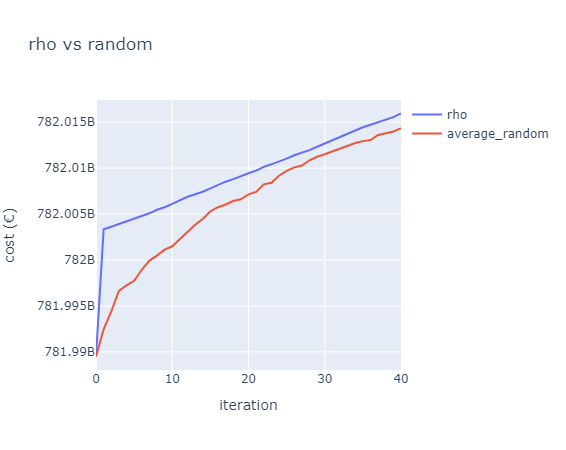
\includegraphics[width=0.8\textwidth]{images/rho_vas_average2.png}
  \caption{Cost variation at each iteration using the \(\rho\) selection method compared to random interval selection.}
  \label{fig:rho_vs_average}
\end{figure}

In plot \ref{fig:val_vs_average}, we compare the cost variation at each iteration using the RH validation method for interval refinement against the random interval selection method. 
The results indicate that the former method yields a significantly faster increase, implying quicker convergence to the optimal solution. 
However, this approach incurs greater computational time: \textcolor{red}{many seconds s}. 
\begin{figure}[htbp]
  \centering
  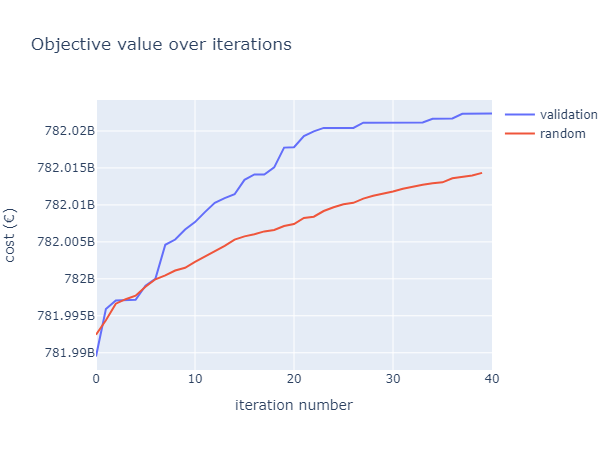
\includegraphics[width=\textwidth]{images/val_vs_average.png}
  \caption{Cost variation at each iteration using the RH validation method for interval refinement against the random interval selection method.}
  \label{fig:val_vs_average}
\end{figure}

It is worth noting that while both the \(\rho\) and random iteration methods continue up until reaching the maximum iteration limit, the RH validation method iteration may halt before that, if the current solution is RH-feasible on the full disaggregated horizon.
The solution found is not necessarily optimal, and other heuristics would then be needed to improve it by readjusting the operational costs of hydrogen conversion and transportation. 
However such adjustments can be made without further increasing the number of disaggregated days, keeping the problem size limited.

Figure \ref{fig:opt_time_over_iter} shows the optimization time across iterations.
 We observe a generally constant, yet slightly decreasing trend in optimization time, indicating that the model is effectively utilizing the warm start. Furthermore, the reduction in optimization time suggests that the number of pivots needed to recover the optimal solution decreases as the optimization progresses, bringing the solution closer to optimality with each iteration.
 While the optimization time remains similar across the different iteration methods, in Figure \ref{fig:iter_time_over_iter} we observe significant variation in the total iteration time. This includes the time spent selecting the time interval to disaggregate, adding additional constraints, and reoptimizing. 
 The validation method performs poorly in this regard due to the time consumed by the RH. However, it is important to note that since the RH method selects intervals one scenario at a time, the iteration time does not depend on the number of scenarios, suggesting that this method could perform well in cases with a large number of scenarios.
 

\begin{figure}[H]
  \centering
  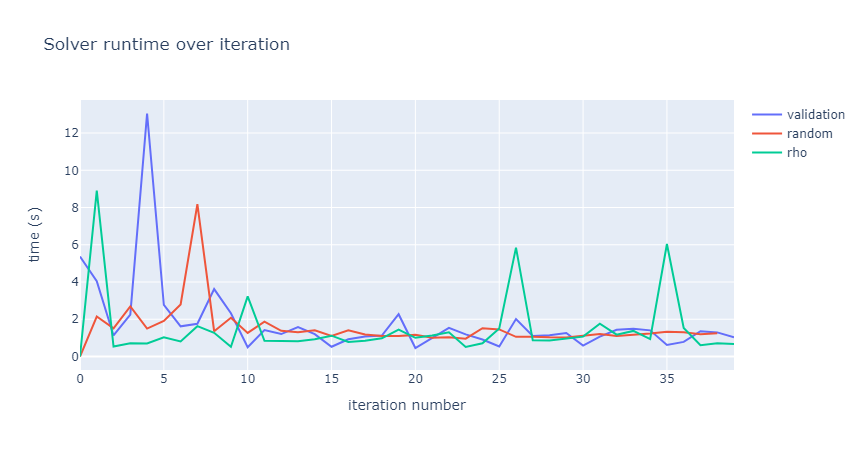
\includegraphics[width=0.85\textwidth]{images/opt_time_over_iter.png}%{images/iter_time_over_iter.png}
  \caption{Solver runtime time over iterations.}
  \label{fig:opt_time_over_iter}
\end{figure}

\begin{figure}[H]
  \centering
  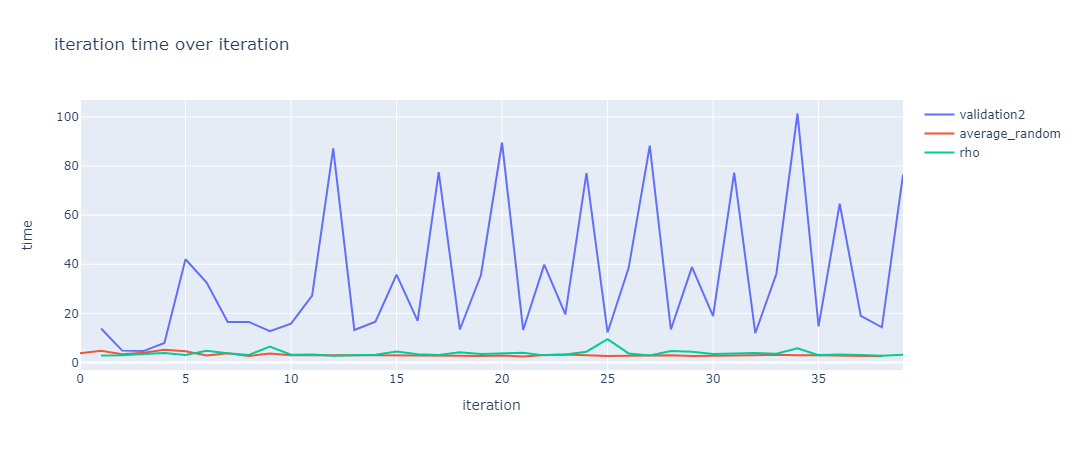
\includegraphics[width=0.85\textwidth]{images/iter_time_over_iter.png}%{images/iter_time_over_iter.png}
  \caption{Iteration time over iterations.}
  \label{fig:iter_time_over_iter}
\end{figure}



\begin{figure}[H]
  \centering
  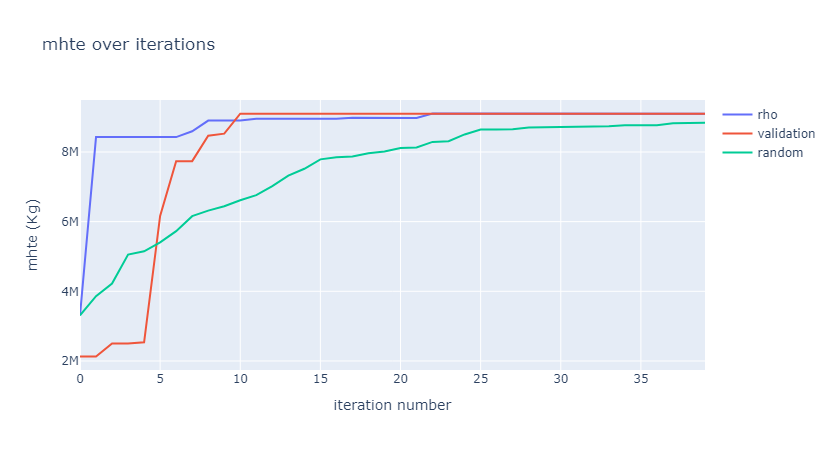
\includegraphics[width=0.85\textwidth]{images/mhte.png}%{images/iter_time_over_iter.png}
  \caption{Iteration time over iterations.}
  \label{fig:iter_time_over_iter}
\end{figure}


%=================================================================================================================================================================================================================================================================================================================
%=================================================================================================================================================================================================================================================================================================================


%=================================================================================================================================================================================================================================================================================================================
%=================================================================================================================================================================================================================================================================================================================








\section{conclusion and Future Directions}

The examples above demonstrate that aggregating time steps, combined with iterative refinement, can effectively solve the Capacity Expansion Problem (CEP). 

We explored two different approaches for selecting time intervals to refine at each iteration. The first approach employed a validation method based on the Rolling Horizon approach, which offers the advantage of providing a feasibility certificate if it halts before reaching the maximum number of iterations and reflects a realistic setting where reliable forecasts for power production are available over a short time span.

The second approach utilized \(\rho\), as defined in Definition \ref{def rho}, representing the fraction of net power production in each time step relative to the total net power production within the corresponding interval. 
The variance of \(\rho\) across each node in the network served as a quality index for each time interval, guiding the disaggregation process by targeting intervals with the worst \(\rho\) values. 
We also provided a theoretical justification for using \(\rho\), explaining that time intervals with greater oscillations in net power production require a finer time partition to be accurately considered, and establishing sufficient conditions under which the aggregated solution can be extended to a feasible solution for the original problem.

The iteration method with RH validation proved to be very effective at selecting relevant intervals to disaggregate. Starting with a day-night aggregation consisting of 730 intervals throughout the year, the method halted on average after \textcolor{red}{XXX} iterations with an RH-feasible solution whose cost diverged only minimally from the optimum.
However, the use of RH within the iteration loop has a non negligible computational cost, granting it does not increase with the number of scenarios. Still, there is a lot of wriggle space in the implementation of this method, which can help further reduce the computational load.

The iteration method with $\rho$ proved more effective than chance at selecting relevant intervals to disaggregate, while maintaining similar computational times.
In future work, we plan to relax the conditions in Proposition \ref{prop rho} for the feasibility of the aggregated solution for the original problem. Furthermore, the interval selection method can be refined by considering other indices based on \(\rho\), such as the frequency of sign changes over time within a time interval, or by using other measures instead of the variance across the nodes of the network.









\color{black}


%\begin{acknowledgements}
%If you'd like to thank anyone, place your comments here
%and remove the percent signs.
%\end{acknowledgements}


% Authors must disclose all relationships or interests that 
% could have direct or potential influence or impart bias on 
% the work: 
%
 \section*{Conflict of interest}
The authors have no competing interests to declare that are relevant to the content of this article.
%
% The authors declare that they have no conflict of interest.


% BibTeX users please use one of
\bibliographystyle{spbasic}      % basic style, author-year citations
%\bibliographystyle{spmpsci} % mathematics and physical sciences
%\bibliographystyle{spphys}       % APS-like style for physics
\bibliography{sample}   % name your BibTeX data base

% Non-BibTeX users please use
% \begin{thebibliography}{}
% %
% % and use \bibitem to create references. Consult the Instructions
% % for authors for reference list style.
% %
% \bibitem{RefJ}
% % Format for Journal Reference
% Author, Article title, Journal, Volume, page numbers (year)
% % Format for books
% \bibitem{RefB}
% Author, Book title, page numbers. Publisher, place (year)
% % etc
% \end{thebibliography}






%=================================================================================================================================================================================================================================================================================================================
%=================================================================================================================================================================================================================================================================================================================

%                                               APPENDIX

%=================================================================================================================================================================================================================================================================================================================
%=================================================================================================================================================================================================================================================================================================================















\newpage
\appendix

\section{Scenario Generation}\label{generation}

To estimate the optimal capacities for the CEP through a stochastic approach, realistic and diverse weather scenarios are needed, so to capture the variability and uncertainty of power generation through renewable sources over extended periods. 
In order to generate such scenarios, samples are extracted from a joint probability density function (PDF) fit on historical data. 
%In the following, we use \(Y_t\) to denote the stochastic process of generated power observations for either solar or wind in a single country.
In our project, we used an hourly time step ($T=8760$) and fit the wind and solar distributions separately for each country considered.

To model the marginal probability distributions corresponding to the power output of wind turbines for each hour of the year, a Weibull distribution was used, justified by its proven effectiveness in capturing the variability and skewness of wind power distributions \citep{weibullwind}. 
For solar power, Beta distributions were employed, as in \citet{betaPV}.
To fit our model, we used a dataset containing 30 years of data for various European countries, which was collected by \citet{30y_gen}. 
On the other hand, electricity load is taken from the \citet{ENTSOE_PowerStats}.
In this simple model, while fitting on historical data we did not account for possible changes in future climate, since the focus lies mostly in the computational aspect.

To account for interdependence between temporally near time steps, we coupled these distributions using a Gaussian Copula approach, which captures the dependencies between hourly power outputs effectively. 
This approach accurately represents the coupled behavior in renewable stochastic systems \citep{GaussCopula}. 

A possible improvement of the generation process could be to fit wind and PV data jointly in the copula step, potentially also including load scenarios with the generation scenarios through the same approach. 
This would consider dependence between Energy Demand and weather conditions, but it would necessitate of the historical dataset provided for the corresponding grid, and would also further increase computational costs.

%\subsubsection{Stochastic Processes description}
%The stochastic processes of power observations will be denoted as \(Y_t\). Where \(t \in T\), is the set indexing all the random variables which want to be considered jointly.
%We assume that the random variable \(Y_t\) has either a Weibull distribution, in the case of Wind Power, or a Beta distribution in the case of Solar Power. 

\subsection{Parametric Estimation of Wind Power distribution}\label{subsection: weib estim}

The parameters defining the Weibull Distribution are estimated using the Maximum Likelyhood Estimation (MLE). 
The Weibull density function is given by:
\begin{equation}
f(x; \theta, \gamma) = \left(\frac{\gamma}{\theta}\right)x^{\gamma-1}\exp\left(-\left(\frac{x}{\theta}\right)^\gamma\right)
\end{equation}
where \(\theta, \gamma > 0\) are the scale and shape parameters, respectively. 

Given observations \(X_1, \ldots, X_n\), the log-likelihood function is:
\begin{equation}
\log L(\theta, \gamma) = \sum_{i=1}^n \log f(X_i \mid \theta, \gamma)
\end{equation}

The optimum solution is found by searching for the parameters for which the gradient is zero:
\begin{equation}
\frac{\partial \log L}{\partial \theta} = -\frac{n \gamma}{\theta} + \frac{\gamma}{\theta^2} \sum_{i=1}^{n} x_i^\gamma = 0
\end{equation}

Eliminating $\theta$, we get:
\begin{equation}
\left[ \frac{\sum_{i=1}^{n} x_i^\gamma \log x_i}{\sum_{i=1}^{n} x_i^\gamma} - \frac{1}{\gamma} \right] = \frac{1}{n} \sum_{i=1}^{n} \log x_i
\end{equation}

This can be solved to get the MLE estimate $\hat{\gamma}$. 
This can be accomplished with the aid of standard iterative procedures such as the Newton-Raphson method or other numerical procedures. 
This is done with the aid of the package \emph{scipy}.
Once $\hat{\gamma}$ is found, $\hat{\theta}$ can be determined in terms of $\hat{\gamma}$ as:
\begin{equation}
\hat{\theta} = \left( \frac{1}{n} \sum_{i=1}^{n} x_i^{\hat{\gamma}} \right)^{\frac{1}{\hat{\gamma}}}
\end{equation}



%%%%%%%%%%%%%%%%%%%%%%%%%%%%%%%%%%%%%%%%%%%%%%%%%%%%%%%%%%%%%%%%%%%%%%%%%%%



\subsection{Parametric Estimation of Solar Power distribution}\label{subsection: beta estim}

To estimate the \(\alpha\) and \(\beta\) parameters defining the Beta distribution \(Y\), we use the Method of Moments.
The mean of the random variable \(Y\) can be expressed as \(\E\left[ Y\right] = \frac{\alpha}{\alpha + \beta} \) and the variance as \(\var [Y]= \frac{\alpha + \beta}{(\alpha + \beta)(\alpha + \beta + 1)}\). 
In particular by explicating \(\beta\) in the first equation and substituting it in the second equation we obtain that:
\begin{equation}
\begin{cases}
\alpha = \mathbb{E}[X] \left( \frac{\mathbb{E}[X](1 - \mathbb{E}[X])}{\mathrm{Var}[X]} - 1 \right) \\
\beta = (1 - \mathbb{E}[X]) \left( \frac{\mathbb{E}[X](1 - \mathbb{E}[X])}{\mathrm{Var}[X]} - 1 \right)
\end{cases}
\end{equation}
By substituting the mean and the variance with their empirical approximation we obtain the Method of Moments estimator for \(\alpha\) and \(\beta\).



%%%%%%%%%%%%%%%%%%%%%%%%%%%%%%%%%%%%%%%%%%%%%%%%%%%%%%%%%%%%%%%%%%%%%%%%%%%



\subsection{Parametric Copula Estimation}
The cumulative density function of both the Weibull and Beta distributions are continuous and invertible. 
Therefore, the random variables \( U_t \coloneqq F_{Y_t}(Y_t) \) have a uniform distribution over \([0,1]\). 
The copula of the random variables \(\{Y_t\}_{t \in T}\) is defined as the function \(C: [0,1]^T \to [0,1]\) such that 
\begin{equation}
C(F_{Y_1}(y_1), \ldots, F_{Y_T}(y_{|T|})) = P(Y_1 \leq y_1, \ldots, Y_{|T|} \leq y_{|T|}).
\end{equation}
This function always exists because of Sklar's Theorem. 
For a given correlation matrix \(\Sigma\), the Gaussian Copula with parameter matrix \(\Sigma\) is defined as 
\[\CG(u_1,\ldots,u_{T}) \coloneqq \Phi_{\Sigma}(\Phi^{-1}(u_1),\ldots, \Phi^{-1}(u_T)),\] 
where \(\Phi,\; \Phi_{\Sigma}\) are the cumulative distribution functions of Gaussian variables having distribution \(\mathcal{N}(0,1)\) and \( \mathcal{N}(\mathbf{0},\Sigma)\) respectively. 
In particular if \(\CG\) is the copula associated with the random variables \(\{Y_t\}_{t \in T}\) then we have that the random variables \(Z_t = \Phi^{-1}(F_{Y_t}(Y_t)) = \Phi^{-1}(U_t)\) have joint distribution equal to \(\mathcal{N}(0, \Sigma)\). 
This follows from:
\begin{align*}
P(Z_1 \leq z_1, \ldots, Z_T \leq z_t) &= P(\Phi^{-1}(U_1) \leq z_1, \ldots, \Phi^{-1}(U_T) \leq z_T) = \\
&= P(U_1 \leq \Phi(z_1), \ldots, U_T \leq \Phi(z_T)) = \\
&= \CG(\Phi(z_1), \ldots, \Phi(z_t)) =  \\
&= \Phi_{\Sigma}(z_1, \ldots, z_T)
\end{align*}
In particular, given the realization \(\{y_{t,j}\}_{t \in t, j \in J}\) of the variables \(\{Y_t\}_{t \in T}\), an unbiased estimation of the parameter matrix \(\Sigma\) is the empirical covariance matrix \(\hat \Sigma\) of the samples \(\{\Phi^{-1}(\hat{F}_{Y_t}(y_{t,j}))\}_{t\in T, j \in J}\), where \(\hat{F}_{Y_t}\) is the estimated marginal distribution of the variable \(Y_t\) obtained as seen in Sections \ref{subsection: weib estim} and \ref{subsection: beta estim}.

Finally, we can generate samples from a Multivariate Gaussian random variable \((Z_{t}, t \in T)\) having distribution \(\mathcal{N}(0, \hat \Sigma)\).
Then the power output scenarios are obtained from these samples by following the previous steps backwards, that is, for each sample, computing \(\hat F_{t}^{-1}(\Phi(Z_{t}))\) for all \(t\in T\). 













%=================================================================================================================================================================================================================================================================================================================
%=================================================================================================================================================================================================================================================================================================================


%=================================================================================================================================================================================================================================================================================================================
%=================================================================================================================================================================================================================================================================================================================
















\section{Structure Preserving Constraint Transformations}\label{appendix B}

Varying time aggregation can be viewed as performing row and column aggregation on the original linear programming (LP) model. Consider the following general linear problem:
\begin{align}
\label{eq:LP}
\min_{x \in \bR^{n}} &c^T x \\ 
\text{s.t.} &\quad Ax = b \\
&x \geq 0
\end{align}

Here, \(A\) is an \(m \times n\) matrix. Now, let \(\rowP = \{\rows_1, \rows_2, \ldots, \rows_{\tilde{n}}\}\) be a partition of \([n]\) (the columns) and \(\colP = \{\cols_1, \cols_2, \ldots, \cols_{\tilde{m}}\}\) a partition of \([m]\) (the rows), corresponding to a partition of the rows and columns of \(A\).

We obtain the corresponding aggregated problem by replacing each set \(\rows\) in \(\rowP\) with a single row, and each set \(R\) in \(\colP\) with a single column. 
One way to aggregate a set of rows (or columns) is by taking a linear combination of the rows (or columns), known as \emph{weighted aggregation}.
We denote the weights of the aggregation by \(\rowW_r\) for \(r \in \rowP\), and \(\colW_c\) for \(c \in \colP\).
The corresponding aggregated LP problem becomes:
\begin{align}
\label{eq:LPaggr}
\min_{\tilde{x} \in \bR^{\tilde{n}}} &\tilde{c}^T \tilde{x} \\ 
\text{s.t.} &\quad \tilde{A} \tilde{x} = \tilde{b} \\ 
&\tilde{x} \geq 0 
\end{align}
where \(\tilde{A}\) is a \(\tilde{m}\times \tilde{n}\) matrix.

In the problem under consideration, we have various types of constraints: Electricity Balance, Hydrogen Balance, Hydrogen Storage, and bounds on the variables. Given a time partition \(P\), we define \(\rowP\) and \(\colP\) such that each set \(S \in \rowP\) corresponds to all constraints of the same type, scenario, and time index \(t\) that falls within the same time interval in \(T\) as \(P\). Similarly, the variables (such as Power generation, Hydrogen generation, etc.) are partitioned in \(\colP\) based on the same criteria.
 Rows and columns are combined via weight aggregation. This aggregation maintains the structure of the original problem, 
meaning that had we formulated the model directly with the aggregated time steps, we would have arrived at the same model.
Before defining a \emph{structure-preserving aggregation} for a general LP, we introduce some notation: 
Given a matrix \(B\) with row and column index sets \(I\) and \(J\), respectively, for any subsets \(I' \subset I\) and \(J' \subset J\), 
we denote the submatrix of \(B\) with rows in \(I'\) and columns in \(J'\) as \(B_{I',J'}\).

Let \(\tilde{A}\) be formed by aggregating the rows and columns of \(A\) according to the partitions \(\rowP\) and \(\colP\), respectively. 
For each \(R \in \rowP\), we denote by \(\tilde{A}_R\) the row in \(\tilde{A}\) resulting from aggregating the rows of \(A\) corresponding to \(R\), 
while \(A_R\) refers to the submatrix of \(A\) consisting of all rows in \(R\). 
Similarly, for each \(C \in \colP\), we define \(\tilde{A}_C\) as the column in \(\tilde{A}\) obtained by aggregating the columns of \(A\) in \(C\), 
and \(A_C\) as the submatrix of \(A\) containing all columns in \(C\). 
Thus, \(\rowP\) and \(\colP\) serve as the index sets for \(\tilde{A}\).

For a family of sets \(F\), we denote the subsets of \(F\) with size exactly \(k\) and greater than \(k\) 
by \(F_{=k}\) and \(F_{>k}\), respectively. 
Specifically, \(\supp(\tilde{A}_R)_{>1} \subset \colP\) represents the set of indices corresponding to partitions 
\(C \in \colP\) with size greater than 1, and \(\supp(A_r)_{>1}\) refers to the set of indices where 
\(c \in C \in \colP\), with \(C\) having a size greater than 1.

\begin{definition}

  \label{def:structure preserving aggregation}
  Given an LP problem \eqref{eq:LP}, we say that a weighted aggregation with respect to partitions \(\rowP, \colP\) is \emph{structure-preserving} if for each \(R \in \rowP\) and each \(r \in R\), there exists \(f^r: [\tilde{n}] \to [n]\)  such that:
  \begin{enumerate}
    \item \label{def:spa bijection}\( f^r|_{\supp(\tilde{A}_{R})}: \supp(\tilde{A}_{R})_{>1} \to \supp(A_{r})_{>1}\) is a bijection such that
    \[\tilde{A}_{R,C} = A_{r,f^r(C)} \text{ for all } C \in \supp(\tilde{A}_{R})_{>1}\].
    \item \label{def: spa injection} If \(f^{r'}(C') = f^r(C)\) then \( C=C'\).
    \item \label{def: spa surjection} \(C = \{f^r(C)\}_{_{r\in R}}\) for all \(R \in \rowP_{>1}\) and \(C \in \colP\). %\(\{f^r(C)\}_{r\in R \in \rowP_{>1}, C \in \colP_{>1}} = \cup_{C \in \colP_{>1}}C\)
  \end{enumerate}
\end{definition}
From condition \ref{def: spa surjection} follows the following:
\begin{observation}
  For all \(\{c\}\in \colP_{=1}\) and constraints \(r \in R \in \rowP_{>1}\), \(f^r(\{c\})= c\).
\end{observation}
{
\color{black}

\begin{example}

  As an example, we consider the function \(f^r\) corresponding to the time step aggregation in CEP as defined in Subsection \ref{subsection: relax}. 
  Let us examine the Power Balance constraints \(r_1\) and \(r_2\) for a fixed node \(n \in \cN\) and time steps \(t_1\) and \(t_2\), 
  where \(T \coloneqq \{t_1, t_2\} \in P\) represents an interval in the time partition of the aggregated problem. 
  We note that both \(f^{r_1}\) and \(f^{r_2}\) satisfy the conditions outlined in Definition \ref{def:structure preserving aggregation}. 
  
  Condition \ref{def: spa bijection} is met as all aggregated variables, \(EtH_T\), \(HtE_T\), and \(P_{l,T}\), 
  are mapped (through violet arrows for \(f^{r_1}\) and blue arrows for \(f^{r_2}\)) to unaggregated variables with the same coefficients.  
  Condition \ref{def: spa surjection} implies that all variables appearing in the two constraints are included in the image of either \(f^{r_1}\) or \(f^{r_2}\). 
  Finally, Condition \ref{def: spa injectction} holds trivially.
\newline
\[
\begin{tikzpicture}
  [place/.style={circle,thick},
  transition/.style={rectangle,draw=black!50,fill=black!20,thick}]

% Nodes for the first two time steps
\node (t1) at (0, 2) {$ES_{t_1}ns + EW_{t_1}nw - EtH_{t_1,0} + HE_{t_1} + P_{l,t_1} = PL_{t_1}$};
\node[circle, minimum size=0.6cm] (nst1) at (-2.6, 2) {};
\node[place] (nwt1) at (-1.2, 2) {};
\node[place] (EtHt1) at (-0.1,  2) {};
\node[place] (HtEt1) at (1.1,  2) {};
\node[circle, minimum size=0.6cm] (Pt1) at (2,  2) {};


\node (t2) at (0, 0) {$ES_{t_2}ns + EW_{t_2}nw - EtH_{t_2,0} + HE_{t_2} + P_{l,t_2} = PL_{t_2}$};
\node[circle, minimum size=0.6cm] (nst2) at (-2.6, 0) {};
\node[place] (nwt2) at (-1.2, 0) {};
\node[place] (EtHt2) at (-0.1,  0) {}; 
\node[place] (HtEt2) at (1.1,  0) {};
\node[circle, minimum size=0.6cm] (Pt2) at (2,  0) {};
% Node for the aggregated constraint
\node (T) at (0, -2) {$(ES_{t_1} + ES_{t_2})ns + (ES_{t_1} + ES_{t_2})nw - EtH_{T} + HtE_{T} + P_{l,T} = PL_{T}$};
\node[place] (nstT) at (-2.4, -2) {};
\node[circle, minimum size=0.6cm] (nwtT) at (0.2, -2) {};
\node[circle, minimum size=0.6cm] (EtHtT) at (1.2, -2) {};
\node[place] (HtEtT) at (2.2, -2) {};
\node[place] (PtT) at (3.3, -2) {};

% Arrows from aggregated constraint to time step 1
\draw[magenta, thick, ->, rounded corners] (nstT) .. controls (-4.5, -1) and (-4.5, 1)  .. node[right, near end] {$\neq$} (nst1);
\draw[magenta, thick, ->, rounded corners] (nwtT) .. controls (-2.6, -1) and (-2.6, 1)  .. node[right, near end] {$\neq$}(nwt1);
\draw[violet, thick, ->, rounded corners] (EtHtT) .. controls (0.3, -1) and (-0.1, 1)  .. node[right, near end] {$=$}(EtHt1);
\draw[violet, thick, ->, rounded corners] (HtEtT) .. controls (2.2, 0) and (1.1, 1)  .. node[right, near end] {$=$}(HtEt1);
\draw[violet, thick, ->, rounded corners] (PtT) .. controls (4.5, -1) and (4, 0.5)  .. node[right, near end] {$=$}(Pt1);
% Arrows from aggregated constraint to time step 2
\draw[cyan, thick, ->, rounded corners] (nstT) .. controls (-2.4, -1.5) and (-2.4, -0.5)  .. node[right] {$\neq$}(nst2);
\draw[cyan, thick, ->, rounded corners] (nwtT) .. controls (-1, -1) and (-1, -0.3)  .. node[right] {$\neq$} (nwt2);
\draw[blue, thick, ->, rounded corners] (EtHtT) .. controls (0.3, -1.5) and (-0.1, -0.5)  .. node[right] {$=$} (EtHt2);
\draw[blue, thick, ->, rounded corners] (HtEtT) .. controls (2.2, -1.5) and (1.1, -0.5)  .. node[right] {$=$}(HtEt2);
\draw[blue, thick, ->, rounded corners] (PtT) .. controls (3.3, -1.5) and (2.5, -0.5)  .. node[right] {$=$}(Pt2);

% Legends for f^t1 and f^t2
\node[below right] at (-4.5, 2) {\textcolor{violet}{\Large $f^{r_1}$}};
\node[below right] at (-3.3, -0.5) {\textcolor{blue}{\Large $f^{r_2}$}};

\end{tikzpicture}
\]
\end{example}
}

% \gr[inline]{
% Per alcune oss le seguenti condizioni si possono togliere: \(f^{r'}(C') = f^r(C) \implies C=C'\) e \(\{f^r(C)\}_{r\in R \in \rowP_{>1}} = \cup_{C \in \colP_{>1}}C\).
% Usiamo entrambe le ipotesi aggiuntive più avanti, la prima ci dice che se mandiamo due variabili \(C,C'\) del problema agregato nella stessa variabile, allora le due variabili iniziali sono la stessa. La seconda che a ogni variabili non agregata corrisponde una variabile aggregata.
% }
\vspace{0.5cm}
This implies that the coefficients of the aggregated variables in the aggregated problem match those
 in the original problem for the corresponding unaggregated variables, \(f^r\) can be seen as a 
 function mapping the aggregated variables to variables of the same "type" in the unaggregated
  constraint.
 While obtaining a feasible solution to \eqref{eq:LP} from \eqref{eq:LPaggr} is not always guaranteed,
  it is possible under certain assumptions.
.
\begin{observation}
\label{ob:aggrconstr}
If \((\rowP, \colP)\) is a structure-preserving aggregation, let \(R \in \rowP\) and \(r \in R\). Let \(\tilde{x}\) be a solution
 to the aggregated problem \eqref{eq:LPaggr}. 
If \(\tilde{b}_r - \tilde{A}_{R, \colP_{=1}} \tilde{x}_{\colP_{=1}} \neq 0\), define 
\[\rho_r \coloneqq \frac{b_r - A_{r, \colP_{=1}} \tilde{x}_{\colP_{=1}}}{\tilde{b}_r
 - \tilde{A}_{R, \colP_{=1}} \tilde{x}_{\colP_{=1}}}.\]
  If \(A_{r, \colP_{=1}} = 0\) and \(b_r = 0\) for all \(r \in R\), then \(\rho_r\) can be chosen arbitrarily. 

If \(\rho_r \geq 0\) and \(x \in \bR^n\) satisfies \(x_{\colP_{=1}} = \tilde{x}_{\colP_{=1}}\) and \(x_{f^r(C)} = \rho_r \tilde{x}_C\) for all \(C \in \supp(\tilde{A}_R)_{>1}\), then \(x\) satisfies the constraint \(A_r x = b_r\) of the original problem.
\end{observation}

\begin{proof}

 Consider, \(A_r x = \sum_{i \in \supp(A_r)} A_{r,i} x_i\). 
  This sum can be divided over the aggregated and unaggregated variables:
  \begin{equation}
    \label{eq:p aggr constr 1}
    A_r x =  A_{r, \colP_{=1}} x_{\colP_{=1}} + \sum_{c \in \supp(A_r)_{>1}}  A_{r, c} x_{c}  .
  \end{equation}
  If \(A_{r, \colP_{=1}} = 0\) and \(b_r = 0\) then \( A_{r, \colP_{=1}} x_{\colP_{=1}} = 0\). Fix \(\rho_r \geq 0\), then
  from the definition of structure-preserving aggregation, we know that \(f^r(\supp(\tilde{A}_R)_{>1}) = \supp(A_r)_{>1}\), so equation \eqref{eq:p aggr constr 1} becomes:
  \begin{equation}
    \label{eq:p aggr constr 2}
    \eqref{eq:p aggr constr 1} = \sum_{S \in \supp(\tilde{A}_R)_{>1}} A_{R, f^r(S)} x_{f^r(S)} =  \sum_{S \in \supp(\tilde{A}_R)_{>1}} \tilde{A}_{R, S} \rho_r \tilde{x}_S  = \rho_r \tilde{A}_R \tilde{x} = 0,
  \end{equation}
  where the second equality holds because \(\tilde{A}_{R, S} = A_{r, f^r(S)}\) and \(x_{f^r(S)} = \rho_r \tilde{x}_S\). Thus, \(x\) satisfies the constraint \(A_r x = b_r\).
  
  When \(A_{r, \colP_{=1}} \neq 0\) or \(b_r \neq 0\), we proceed similarly:
  \begin{align}
  \label{eq:p aggr constr 3}
 \eqref{eq:p aggr constr 1} &=A_{r, \colP_{=1}} x_{\colP_{=1}} + \sum_{S \in \supp(\tilde{A}_R)_{>1}} A_{r, f^r(S)} x_{f^r(S)}  \\
  &=  A_{r, \colP_{=1}} \tilde{x}_{\colP_{=1}} + \rho_r \sum_{S \in \supp(\tilde{A}_R)_{>1}} \tilde{A}_{R, S}  \tilde{x}_S.
  \end{align}
  
  By the definition of \(\rho_r\) the second sum in the last line of equation \eqref{eq:p aggr constr 3} is equal to:
  \begin{align*}
  \rho_r \sum_{S \in \supp(\tilde{A}_R)_{>1}} \tilde{A}_{R, S} \tilde{x}_S 
  &= \rho_r (\tilde{A}_R \tilde{x} - \tilde{A}_{R, \colP_{=1}} \tilde{x}_{\colP_{=1}}) \\
  &= \rho_r (\tilde{b}_R - \tilde{A}_{R, \colP_{=1}} \tilde{x}_{\colP_{=1}}) \\
  &= b_r - A_{r, \colP_{=1}} \tilde{x}_{\colP_{=1}}.
  \end{align*}
  
  Thus, we obtain:
  \[
  A_r x = b_r.
  \]
  \qed
  \end{proof}


A structure-preserving aggregation does not inherently ensure the feasibility of all constraints in the original problem. However, Observation \ref{ob:aggrconstr} demonstrates how to partially reconstruct a solution \(x\) for a specific constraint \(r\) by scaling the aggregated variables appropriately within the support of \(A_r\).

\begin{definition}
  Let \(\rho_r\) be defined as in Observation \ref{ob:aggrconstr} for all \(r \in R \in \rowP_{>1}\). Let \(x \in \bR^n\) be defined as \(x_{\colP_{=1}} \coloneqq \tilde{x}_{\colP_{=1}}\) and \(x_{f^r(C)} \coloneqq \rho_r \tilde{x}_C\) for all \(C \in \colP_{>1}\) and \(r \in R \in \rowP_{>1}\). Then \(x\) is well defined if for all \(r, r' \in R \in \rowP_{>1}\) such that \(f^r(C) = f^{r'}(C)\), we have \(\rho_r = \rho_{r'}\). In such case we refer to \(x\) as a \(rho\)-solution. 
\end{definition}

If \(x\) is a \(\rho\)-solution.  \(x\) is a feasible solution for the constraints in \(\rowP_{>1}\), we also need to ensure that \(x\) is also feasible for the remaining constraints in \(\rowP_{=1}\).

 

% \begin{definition}
%   For a structure-preserving, row and column aggregation \((\rowP,\colP)\).
%   A constraint \(r \in \colP_{=1}\) is \(\rho\)-agnostic if for all the feasible solution \(\tilde{x}\) of the aggregated problem all \(\rho \in \bR^{\cup_{R \in \rowP_{>1}} R}\) such that 
%   \(\omega_R^T\rho_R = 1\) for all \(R \in \rowP_{>1}\) then \(x\) defined as in Observation \ref{ob:aggrconstr} is well defined.
% \end{definition}

\begin{example}
  Consider the constraint that the initial hydrogen stored must be equal to the final hydrogen stor for a one node network:
  \begin{equation}
    \label{eq:examplehydrogen}
    \sum_{t=1}^n \Delta H_t = 0
  \end{equation}
  The corresponding aggregated constraint is for a time partition \(P\) is:
  \begin{equation}
    \sum_{T \in P} \Delta H_T = 0
  \end{equation}
  For all \(\rho\) such that \(\sum_{t\in T}\rho_t = 1\) for all \(T\) in \(P\), given a feasible solution for the aggregated problem \(\tilde{\Delta H_T}\), let \(\Delta H_t \coloneqq \rho_t \tilde{\Delta H_T}\), then constraint \eqref{eq:examplehydrogen} holds: 
  \begin{equation}
    \sum_{t=1}^n \Delta{H_t} = \sum_{t=1}^n \rho_t \tilde{\Delta H_T} = \sum_{T \in P} \sum_{t\in T} \rho_t \tilde{\Delta H_T} = \sum_{T \in P} \tilde{ \Delta H_T} = 0
  \end{equation}
  Thus constraint \eqref{eq:examplehydrogen}is holds for \(\rho\)-solutions
\end{example}

This is a special instance of a general class of constraints that always hold for \(\rho\)-solutions, this follows from the following propriety of \(\rho\)-solutions:

\begin{observation}
  \label{ob:rhoconvex}
  Let \(\rowW_r \in \bR\) for all \(r \in R \in \rowP\) be the weights of the row aggregation.
  If \(x\) is a \(\rho\)-solution, then we have, for all \(R \in \rowP_{>1}\):
  \begin{equation}
    \rowW_R^T \rho_R = 1
  \end{equation}
\end{observation}
\begin{proof}
  \[
  \rowW_R^T \rho_R = \sum_{r \in R} \rowW_r \rho_r =  \frac{\sum_{r \in R}\rowW_r(b_r - A_{r, \colP_{=1}} \tilde{x}_{\colP_{=1}})}{\tilde{b}_r
  - \tilde{A}_{R, \colP_{=1}} \tilde{x}_{\colP_{=1}}} = 1
  \] 
\end{proof}
Note that if \(x\) is a \(\rho\)-solution, then for all \(C \in \supp(A_{r})_{>1}\), we can pick \(R^{(C)} \in \rowP_{>1}\) so that \(C \in \supp(\tilde{A}_{R^{(C)}})\) and \(x_{f^r(C)} = \rho_r \tilde{x}_C\) for all \(r \in R^{(C)}\) and the definition of \(x\) does not depend on the choice of \(R^{(C)}\).
\begin{observation}
  Le \((\rowP,\colP)\) be a structure-preserving, row and column aggregation. If \(x\) is a \(\rho\)-solution and \(r\) is a constraint in \(\rowP_{=1}\), such that 
  \[A_{r,f^{r'}(C)} = \rowW_{r'}\tilde{A}_{r,C} \text{ for all } r' \in R^{(C)},\; C \in \colP_{>1}, \]
  then \(x\) is a fesible solution for constraint \(r\).
\end{observation}

\begin{proof}
As before we split the sum \(A_rx\) over aggregated and unaggregated variables:
\begin{equation}
  \label{eq:rho agn eq1}
  A_rx = \sum_{C \in \colP_{=1}}A_{r,C}x_{C} +  \sum_{C \in \supp(A_{r})_{>1}} \sum_{r' \in R^{(C)}} A_{r,f^{r'}(C)}x_{f^{r'}(C)}
\end{equation}
From the hypothesis and the definition of \(\rho\)-solution, we have:
\begin{equation}
  \label{eq:rho agn eq2}
    \eqref{eq:rho agn eq1} =  \sum_{C \in \colP_{=1}}\tilde{A}_{r,C}\tilde{x}_{r,C} +  \sum_{C \in \supp(A_{r})_{>1}} \sum_{r' \in R^{(C)}}\rowW_{r'} \tilde{A}_{r,C}\rho_{r'}\tilde{x}_{C} 
\end{equation}
Since \(\rowW_{R^{(C)}} \rho_{R^{(C)}} = 1\), we have
\begin{equation}
  \label{eq:rho agn eq3}
    \eqref{eq:rho agn eq2} =   \sum_{C \in \colP_{=1}}\tilde{A}_{r,C}\tilde{x}_{r,C} +  \sum_{C \in \supp(A_{r})_{>1}}\tilde{A}_{r,C}\tilde{x}_{C} = \tilde{A}_r\tilde{x}_r = \tilde{b}_r = b_r
\end{equation}
\end{proof}

We now define the hypergraph associated to the aggregation \((\rowP, \colP)\).
\begin{definition}
  The \emph{hypergraph associated to the aggregation \((\rowP, \colP)\)} is the hypergraph \(\cN, \cE\) having as nodes the unaggregated variables in  \(\cN \coloneqq \colP_{>1}\) and as edges the subsest of \(\cN\) that appear together in constraints in \(\rowP_{>1}\).
\end{definition}

When two edges (constraints) in the hypergraph, \(r\) and \(r'\), share aggregated variables, 
the scaling factors \(\rho_r\) and \(\rho_{r'}\) must be equal for Observation \ref{ob:aggrconstr} to hold for both \(r\) and \(r'\). 
From this follows the following:
\begin{proposition}
\label{prop:xaggfeasible}
If \((\rowP, \colP)\) is a structure-preserving aggregation and the constraints in \(\rowP_{=1}\) hold for \(rho\)-solutions. Let \(\tilde{x}\) be a solution 
to the aggregated problem \eqref{eq:LPaggr}. For all \(r \in R \in \rowP_{>1}\) define \(\rho_r\) as in Observation \ref{ob:aggrconstr}. If \(\rho_r \geq 0\) and is constant over the connected components of the hypergraph associated to \((\rowP, \colP)\). 
Then \(x_{\colP_{=1}} \coloneqq \tilde{x}_{\colP_{=1}}\) and \(x_{f^r(C)} \coloneqq \rho_r \tilde{x}_C\) for all \(C \in \supp(\tilde{A}_R)\) and \(C \in \colP_{>1}\) is well defined and thus \(x\) is a \(\rho\)-solution.
Further more if \(x\) is feasible for all constraints in \(\colP_{=1}\), then \(x\) is feasible solution to the unaggregated problem \eqref{eq:LP}.
\end{proposition}

Until now we have only considered feasibility, ignoring the relationship between the cost of \(\tilde{x}\) and the cost of \(x\). The following observation gives a condition for the cost of \(\tilde{x}\) to be equal to the cost of \(x\).
For all \(C \in \colP_{>1}\) let  \(R^{(C)} \in \rowP_{>1}\) be so that \(C \in \supp(\tilde{A}_{R^{(C)}})\) and \(x_{f^r(C)} = \rho_r \tilde{x}_C\) for all \(r \in R^{(C)}\).
\begin{observation}
  \label{ob:costpreserving}
  Let \(x\) be a \(\rho\)-solution. If  \(\rowW_r\tilde{c}_C = c_{f(r,C)}\) for all \(r \in R^{(C)} \in \rowP_{>1}\), then the cost of \(\tilde{x}\) for the aggregated problem 
  is equal to the cost of \(x\) in the unaggregated problem. 
\end{observation}
\begin{proof}
  Let \(\tilde{x}\) be a solution to the aggregated problem \eqref{eq:LPaggr}. Using Observation \ref{ob:rhoconvex}, for all \(C \in \colP_{>1}\) the cost corresponding to the variable \(\tilde{x}_C\) is 
  \[
  \tilde{c}_C\tilde{x}_C = \tilde{c}_C(\sum_{r \in R^{(C)}}\rowW_r\rho_r)\tilde{x}_C = \sum_{r \in R^{(C)}}\tilde{c}_C\rowW_r\rho_r\tilde{x}_C  = \sum_{r \in R^{(C)}}c_{f(r,C)}x_{f(r,C)}
  \]
  Which corresponds to the cost of the variables \(\{x_{f(r,C)}\}_{r \in R^{(C)}}\). Thus
  \begin{align*}
  \tilde{c}\tilde{x} &= \sum_{C \in \colP_{=1}}\tilde{c}_C\tilde{x}_C + \sum_{C \in \colP_{>1}}\tilde{c}_C\tilde{x}_C \\
                    &= \sum_{C \in \colP_{=1}}c_Cx_C + \sum_{C \in \colP_{>1}}\sum_{r \in R^{(C)}}c_{f(r,C)}x_{f(r,C)} \\
                    &= \sum_{C \in \colP_{=1}}c_Cx_C + \sum_{j \in \cup_{C \in \colP_{>1}}C}c_{j}x_{j} \\
                    &= cx
  \end{align*}
\qed
\end{proof}


While row aggregation of a linear problem is a relaxation of the original problem, the same does not apply to column aggregation. However, the column aggregation used for the  Capacity Expansion Problem in this work is still a relaxation. In general a column aggregation of a linear problem is a relaxation of the original problem whenever it is a \emph{constant-coefficients column aggregation}, that is:
\begin{definition}
  A column aggregation of a linear problem, respect to the column partition \(\colP\), is a \emph{constant-coefficients column aggregation} if, for all \(C \in \colP_{>1}\), the non-zero rows in \(A_C\) are identical.
\end{definition}

\begin{proposition}
If \((\rowP,\colP)\) is a structure-preserving, constant-coefficients column aggregation,
if the hypothesis of Proposition \ref{prop:xaggfeasible} and Observation \ref{ob:costpreserving} are true, then the aggregated problem \eqref{eq:LPaggr} is exact and the \(\rho\)-solution \(x\) is an optimal solution.
\end{proposition}

% \begin{proof}
   Since for Observation \ref{ob:costpreserving}, the cost of the aggregated problem is equal to the cost of \(x\) in the unaggregated problem, we only need that the aggregated problem is a relaxation of the unaggregated problem.
   But this is true since both row aggregations and constant-coefficients column aggregations are are relaxations.
%   Let \(x\) be a solution to the unaggregated problem \eqref{eq:LP}. For all \(C \in \colP_{=1}\) let \(\tilde{x}_C \coloneqq x_C\).
%   Since  \(\{f^r(C)\}_{r \in \cup_{R\in \rowP_{>1}}, C \in \colP} = \cup_{C \in \colP_{>1}}C\), for all \(c \in C \in \colP_{>1}\), exists \(r \in R \in \rowP_{>1}\) and \(C \in \colP_{>1}\) such that \(f^r(C) = c\).
%   Then let \(\tilde{x}_C \coloneqq \sum_{c \in C}A_{r,c}x_c\). Since if \(f^{r}(C)= f^{r'}(C')\) implies that \(C=C'\), \(x\) is well defined.
%   Lastly for all \(R \in \rowP\) we have:
%   \[\tilde{A}_R\tilde{x} = \sum_{r \in R} \left( \sum_{C \in \colP_{=1}}\rowW_rA_{r,c}\tilde{x}_C + \sum_{C\in \supp(\tilde{A}_r)_{>1}} \tilde{x}_C \right) = \sum_{r \in R} \left( \sum_{C \in \colP_{=1}}\rowW_rA_{r,c}x_C + \sum_{C\in \supp(\tilde{A}_r)_{>1}} \sum_{c \in C}A_{r,c}x_c \right) = \sum_{r \in R} \tilde{\rho_r} b_r = \tilde{b}_R 
%   \]
%   \qed
% \end{proof}










\end{document}
% end of file template.tex

